\FloatBarrier
\section{\texorpdfstring{$N$-body Problems}{N-body Problems}} \label{sec:Nbody}

Under the framework of the method of regularised stokeslets, using the standard boundary integral method, the evaluation of velocities at $N$ locations in this fluid caused by $N$ force points boils down to an $N$-body problem where if computed exactly through the use of the direct product (eq.~\ref{eq:matrixvectorproduct}) requires $\mathcal{O}(N^2)$ calculations. For a large number of particles, the computation time quickly becomes prohibitive due to rapid growth in the number of operations as the number of particles increases. With the rise of more powerful computers, and the need to compute problems with larger number of interactions, fast algorithms for the summation of particle to particle interactions have been developed which aim to reduce the number of calculations needed to solve problems. 

$N$-body problems of the form
\begin{equation*}
    \bm{u}(\bm{x}_i) = \sum_{n=1}^N \Phi(\bm{x}_n,{\bm{x}}_n){\bm{f}}_n
\end{equation*}
where $\Phi$ is the Green's function associated with the underlying partial differential equation governing the dynamics of the system arise in many problems from electrostatics \cite{Beatson,Tornberg2008}, heat conduction \cite{Greengard1990APotentials}, Stokes flow \cite{Cortez2015,Tornberg2008} and stellar dynamics \cite{Dehnen2014ADynamics}. Most methods of fast summation utilise tree based grouping of the particles in order to form clusters of particles in which the particle to particles can be computed quickly and efficiently. 

In this section we will explore the development of tree based algorithms for the fast summation of $N$-body problems, in particular the Barnes-Hut method \cite{Barnes1986} \cref{subsec:BarnesHut} which provides an easily implemented method for solving $N$-body systems and an $\mathcal{O}(N\log N)$ complexity for the summation. From the Barnes-Hut method we will explore how Greengard and Rokhlin \cite{1988The0-262-7110-X.,Rokhlin1985RapidTheory,Greengard1987ASimulations} adapted the Barnes-Hut method to create analytically correct results while still retaining $\mathcal{O}(N\log N)$ complexity by using multipole expansions (\cref{subsec:ExactNlogN}). The use of multipole expansion was later expanded by Greengard, Rokhlin and Beatson \cite{Beatson,Greengard1987ASimulations} to create an analytically correct algorithm with complexity $\mathcal{O}(N)$ called the Fast Mutlipole Method (FMM). We will explore briefly how these multipole expansion can be used in the 2D case of the Coulombs potential in order to illustrate the ideas behind the algorithm. However, due to the need to form factorisations of the kernel which are not easily obtained of the method of regularised stokeslets, although can be obtained for singular Stokelet and Stresslet kernels \cref{eq:singularsolutions} \cite{Tornberg2008}, we need to consider a kernel independent method. In \cref{sec:KIFMM} we will review the Kernel Independent Fast Multipole Method (KIFMM) created by Ying, Biros and Zorin \cite{Ying2004}, and how it can be adapted for use with the method of regularised stokeslets. 

We will also consider in \cref{sec:NEAREST} an adaption to the Nyström method based on nearest neighbour interpolation which reduces the overall size of the system and decouples $\epsilon$ from the force quadrature spacing $h$. This method provides a easy method to reduce the overall number of particles which need to be considered when solving problems such as resistance problems (\cref{sec:resistance}) or swimming problems (\cref{sec:swimming}).
We will also consider a hybrid implentation of the KIFMM and NEAREST method and explore its use in \cref{sec:NumericalSims}. Due to the single direction of the computation of FMM algorithms we will also explore how the GMRES algorithm can be used with this hybrid method to solve large swimming problems including the derivations of an appropriate preconditioner.  

\subsection{Barnes-Hut Method} \label{subsec:BarnesHut}
One of the first methods proposed to compute $N$-body systems was that of Barnes and Hut \cite{Barnes1986} and is a tree-based method for the computation of $N$-body simulations. By using a Quadtree in two dimensions \cref{fig:2DDecompostion} or octtree in three dimensions \cref{fig:Decompostionexample} the number of computations needed in the $N$-body problem is reduced to $\mathcal{O}(N\log N)$. Tree-based decomposition uses a tree data structure to `bin' particles in smaller domains in which we can consider particle to particle interactions for particles close to each other and an approximation of the particle for particles further away. 


\subsection{Tree-Based Decomposition} \label{sec:TreeDecomp}

\begin{figure}
    \begin{subfigure}[b]{0.4\textwidth}
        \centering
        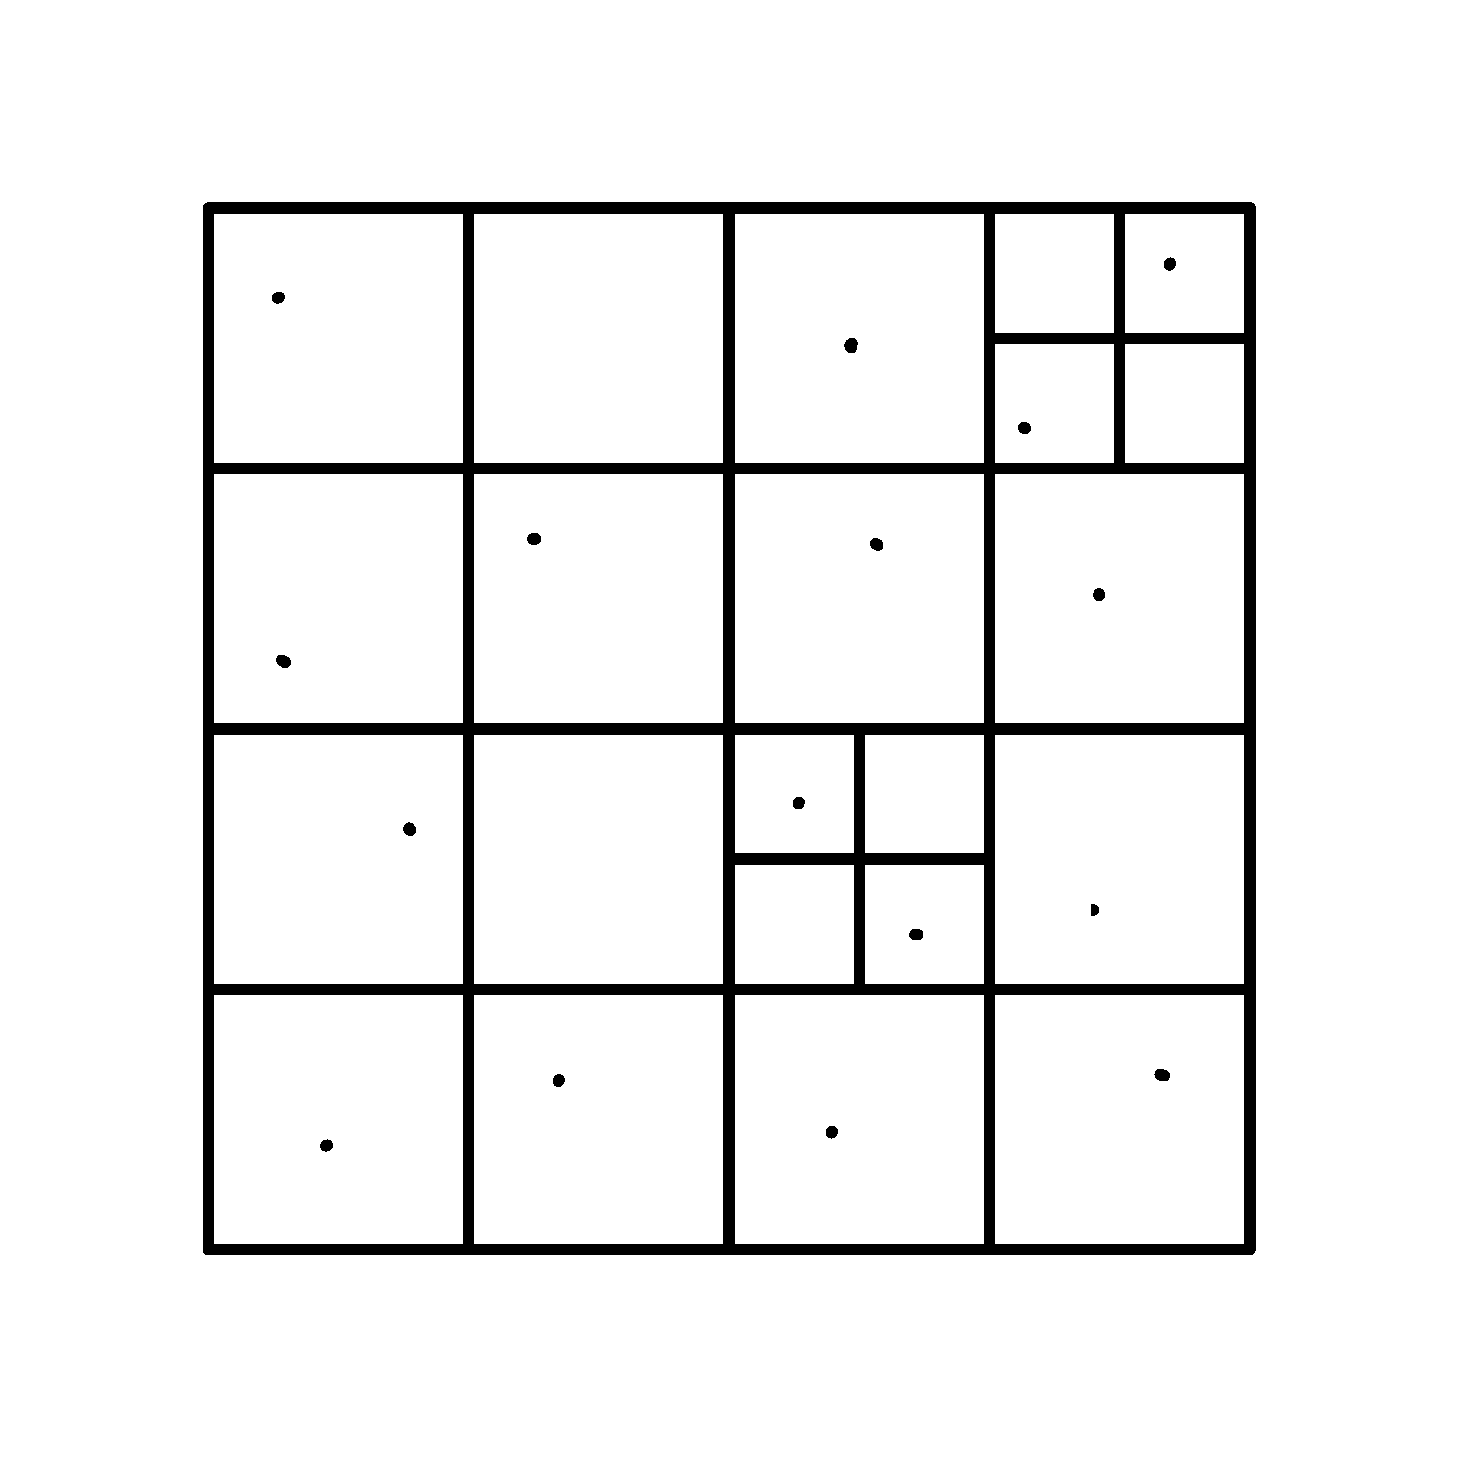
\includegraphics[width=\textwidth]{Images/KIFMM/Decomposition.pdf}
        \caption{\label{fig:2DDecompostion}}
    \end{subfigure}
    \hfill
    \begin{subfigure}[b]{0.4\textwidth}
    \centering
        \resizebox{\linewidth}{!}{% This file was created by matlab2tikz.
%
%The latest updates can be retrieved from
%  http://www.mathworks.com/matlabcentral/fileexchange/22022-matlab2tikz-matlab2tikz
%where you can also make suggestions and rate matlab2tikz.
%
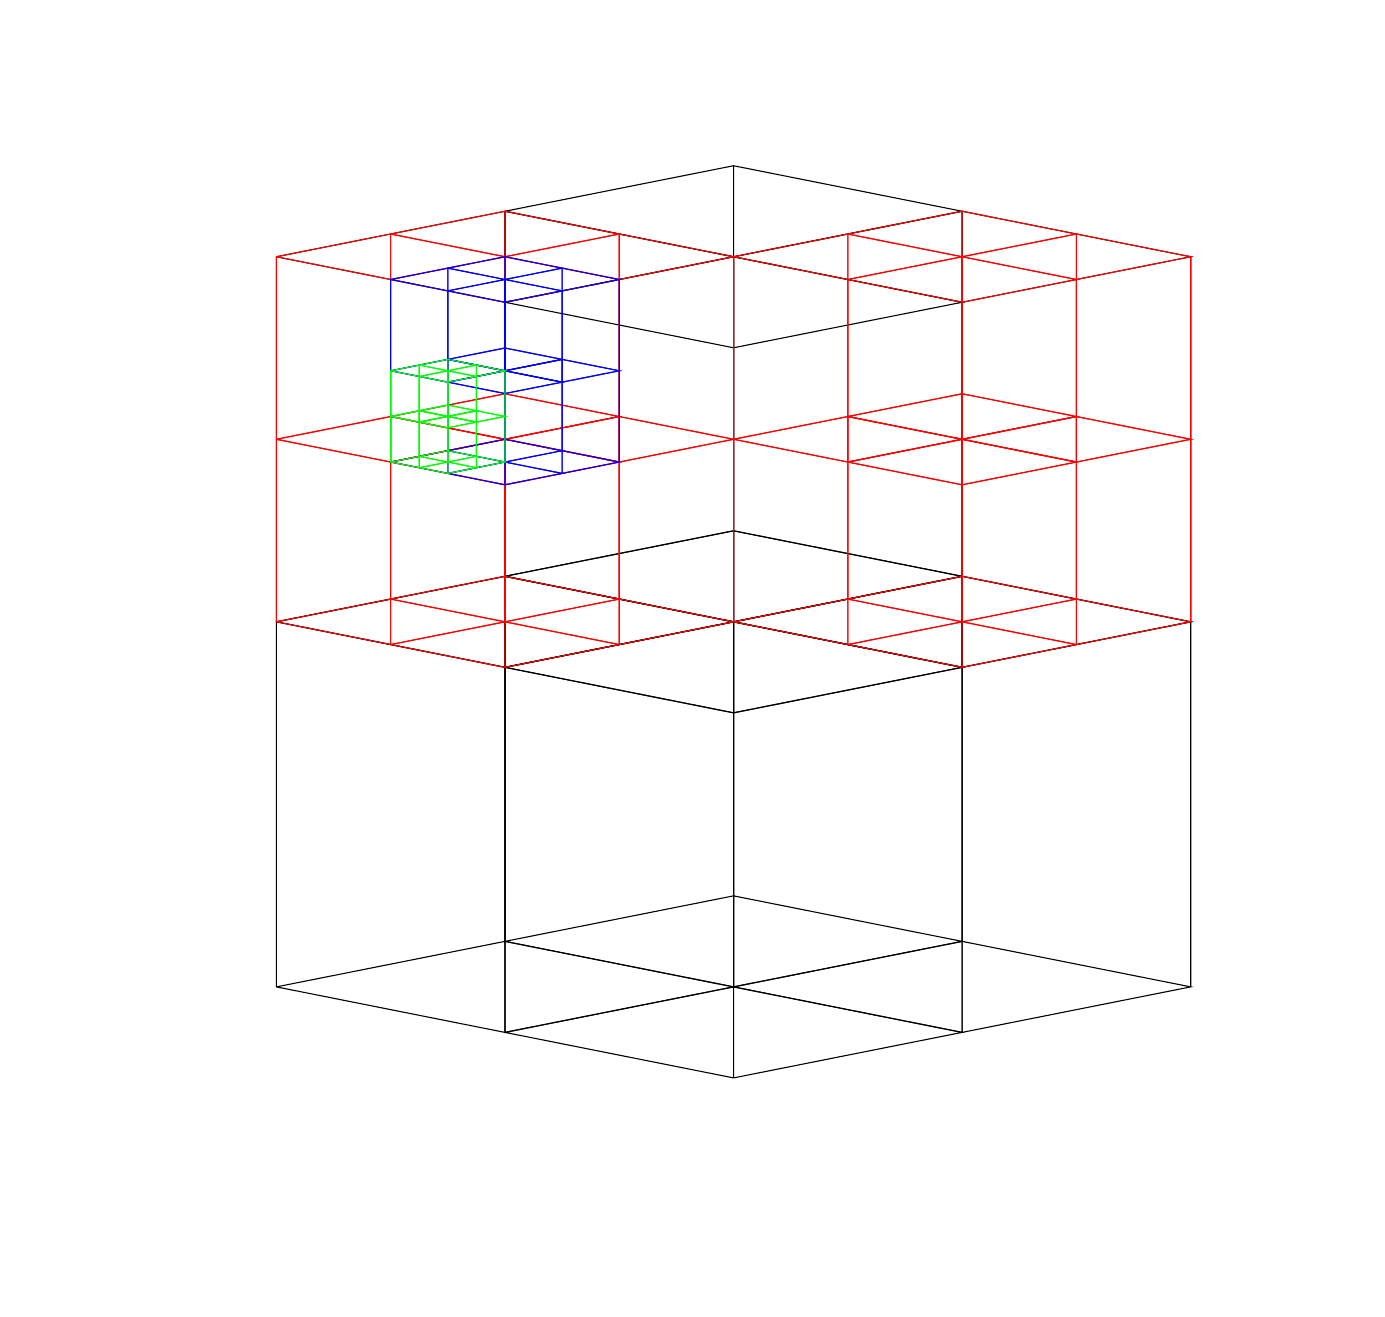
\begin{tikzpicture}

\begin{axis}[%
width=5.151in,
height=5.139in,
at={(0.864in,0.694in)},
scale only axis,
unbounded coords=jump,
xmin=0,
xmax=1,
tick align=outside,
ymin=0,
ymax=1,
zmin=0,
zmax=1,
view={45}{10},
axis line style={draw=none},
ticks=none,
axis x line*=bottom,
axis y line*=left,
axis z line*=left
]
\addplot3 [color=black]
 table[row sep=crcr] {%
0.0737015537421595	0.0737015537421595	0.0737015537421595\\
0.517448266926349	0.0737015537421595	0.0737015537421595\\
0.517448266926349	0.517448266926349	0.0737015537421595\\
0.0737015537421595	0.517448266926349	0.0737015537421595\\
0.0737015537421595	0.0737015537421595	0.0737015537421595\\
0.0737015537421595	0.0737015537421595	0.517448266926349\\
0.517448266926349	0.0737015537421595	0.517448266926349\\
0.517448266926349	0.517448266926349	0.517448266926349\\
0.0737015537421595	0.517448266926349	0.517448266926349\\
0.0737015537421595	0.0737015537421595	0.517448266926349\\
0.0737015537421595	0.0737015537421595	0.0737015537421595\\
nan	nan	nan\\
0.517448266926349	0.0737015537421595	0.0737015537421595\\
0.517448266926349	0.0737015537421595	0.517448266926349\\
nan	nan	nan\\
0.517448266926349	0.517448266926349	0.0737015537421595\\
0.517448266926349	0.517448266926349	0.517448266926349\\
nan	nan	nan\\
0.0737015537421595	0.517448266926349	0.0737015537421595\\
0.0737015537421595	0.517448266926349	0.517448266926349\\
};
 \addplot3 [color=black]
 table[row sep=crcr] {%
0.0737015537421595	0.0737015537421595	0.517448266926349\\
0.517448266926349	0.0737015537421595	0.517448266926349\\
0.517448266926349	0.517448266926349	0.517448266926349\\
0.0737015537421595	0.517448266926349	0.517448266926349\\
0.0737015537421595	0.0737015537421595	0.517448266926349\\
0.0737015537421595	0.0737015537421595	0.961194980110539\\
0.517448266926349	0.0737015537421595	0.961194980110539\\
0.517448266926349	0.517448266926349	0.961194980110539\\
0.0737015537421595	0.517448266926349	0.961194980110539\\
0.0737015537421595	0.0737015537421595	0.961194980110539\\
0.0737015537421595	0.0737015537421595	0.517448266926349\\
nan	nan	nan\\
0.517448266926349	0.0737015537421595	0.517448266926349\\
0.517448266926349	0.0737015537421595	0.961194980110539\\
nan	nan	nan\\
0.517448266926349	0.517448266926349	0.517448266926349\\
0.517448266926349	0.517448266926349	0.961194980110539\\
nan	nan	nan\\
0.0737015537421595	0.517448266926349	0.517448266926349\\
0.0737015537421595	0.517448266926349	0.961194980110539\\
};
 \addplot3 [color=black]
 table[row sep=crcr] {%
0.0737015537421595	0.517448266926349	0.0737015537421595\\
0.517448266926349	0.517448266926349	0.0737015537421595\\
0.517448266926349	0.961194980110539	0.0737015537421595\\
0.0737015537421595	0.961194980110539	0.0737015537421595\\
0.0737015537421595	0.517448266926349	0.0737015537421595\\
0.0737015537421595	0.517448266926349	0.517448266926349\\
0.517448266926349	0.517448266926349	0.517448266926349\\
0.517448266926349	0.961194980110539	0.517448266926349\\
0.0737015537421595	0.961194980110539	0.517448266926349\\
0.0737015537421595	0.517448266926349	0.517448266926349\\
0.0737015537421595	0.517448266926349	0.0737015537421595\\
nan	nan	nan\\
0.517448266926349	0.517448266926349	0.0737015537421595\\
0.517448266926349	0.517448266926349	0.517448266926349\\
nan	nan	nan\\
0.517448266926349	0.961194980110539	0.0737015537421595\\
0.517448266926349	0.961194980110539	0.517448266926349\\
nan	nan	nan\\
0.0737015537421595	0.961194980110539	0.0737015537421595\\
0.0737015537421595	0.961194980110539	0.517448266926349\\
};
 \addplot3 [color=black]
 table[row sep=crcr] {%
0.0737015537421595	0.517448266926349	0.517448266926349\\
0.517448266926349	0.517448266926349	0.517448266926349\\
0.517448266926349	0.961194980110539	0.517448266926349\\
0.0737015537421595	0.961194980110539	0.517448266926349\\
0.0737015537421595	0.517448266926349	0.517448266926349\\
0.0737015537421595	0.517448266926349	0.961194980110539\\
0.517448266926349	0.517448266926349	0.961194980110539\\
0.517448266926349	0.961194980110539	0.961194980110539\\
0.0737015537421595	0.961194980110539	0.961194980110539\\
0.0737015537421595	0.517448266926349	0.961194980110539\\
0.0737015537421595	0.517448266926349	0.517448266926349\\
nan	nan	nan\\
0.517448266926349	0.517448266926349	0.517448266926349\\
0.517448266926349	0.517448266926349	0.961194980110539\\
nan	nan	nan\\
0.517448266926349	0.961194980110539	0.517448266926349\\
0.517448266926349	0.961194980110539	0.961194980110539\\
nan	nan	nan\\
0.0737015537421595	0.961194980110539	0.517448266926349\\
0.0737015537421595	0.961194980110539	0.961194980110539\\
};
 \addplot3 [color=black]
 table[row sep=crcr] {%
0.517448266926349	0.0737015537421595	0.0737015537421595\\
0.961194980110539	0.0737015537421595	0.0737015537421595\\
0.961194980110539	0.517448266926349	0.0737015537421595\\
0.517448266926349	0.517448266926349	0.0737015537421595\\
0.517448266926349	0.0737015537421595	0.0737015537421595\\
0.517448266926349	0.0737015537421595	0.517448266926349\\
0.961194980110539	0.0737015537421595	0.517448266926349\\
0.961194980110539	0.517448266926349	0.517448266926349\\
0.517448266926349	0.517448266926349	0.517448266926349\\
0.517448266926349	0.0737015537421595	0.517448266926349\\
0.517448266926349	0.0737015537421595	0.0737015537421595\\
nan	nan	nan\\
0.961194980110539	0.0737015537421595	0.0737015537421595\\
0.961194980110539	0.0737015537421595	0.517448266926349\\
nan	nan	nan\\
0.961194980110539	0.517448266926349	0.0737015537421595\\
0.961194980110539	0.517448266926349	0.517448266926349\\
nan	nan	nan\\
0.517448266926349	0.517448266926349	0.0737015537421595\\
0.517448266926349	0.517448266926349	0.517448266926349\\
};
 \addplot3 [color=black]
 table[row sep=crcr] {%
0.517448266926349	0.0737015537421595	0.517448266926349\\
0.961194980110539	0.0737015537421595	0.517448266926349\\
0.961194980110539	0.517448266926349	0.517448266926349\\
0.517448266926349	0.517448266926349	0.517448266926349\\
0.517448266926349	0.0737015537421595	0.517448266926349\\
0.517448266926349	0.0737015537421595	0.961194980110539\\
0.961194980110539	0.0737015537421595	0.961194980110539\\
0.961194980110539	0.517448266926349	0.961194980110539\\
0.517448266926349	0.517448266926349	0.961194980110539\\
0.517448266926349	0.0737015537421595	0.961194980110539\\
0.517448266926349	0.0737015537421595	0.517448266926349\\
nan	nan	nan\\
0.961194980110539	0.0737015537421595	0.517448266926349\\
0.961194980110539	0.0737015537421595	0.961194980110539\\
nan	nan	nan\\
0.961194980110539	0.517448266926349	0.517448266926349\\
0.961194980110539	0.517448266926349	0.961194980110539\\
nan	nan	nan\\
0.517448266926349	0.517448266926349	0.517448266926349\\
0.517448266926349	0.517448266926349	0.961194980110539\\
};
 \addplot3 [color=black]
 table[row sep=crcr] {%
0.517448266926349	0.517448266926349	0.0737015537421595\\
0.961194980110539	0.517448266926349	0.0737015537421595\\
0.961194980110539	0.961194980110539	0.0737015537421595\\
0.517448266926349	0.961194980110539	0.0737015537421595\\
0.517448266926349	0.517448266926349	0.0737015537421595\\
0.517448266926349	0.517448266926349	0.517448266926349\\
0.961194980110539	0.517448266926349	0.517448266926349\\
0.961194980110539	0.961194980110539	0.517448266926349\\
0.517448266926349	0.961194980110539	0.517448266926349\\
0.517448266926349	0.517448266926349	0.517448266926349\\
0.517448266926349	0.517448266926349	0.0737015537421595\\
nan	nan	nan\\
0.961194980110539	0.517448266926349	0.0737015537421595\\
0.961194980110539	0.517448266926349	0.517448266926349\\
nan	nan	nan\\
0.961194980110539	0.961194980110539	0.0737015537421595\\
0.961194980110539	0.961194980110539	0.517448266926349\\
nan	nan	nan\\
0.517448266926349	0.961194980110539	0.0737015537421595\\
0.517448266926349	0.961194980110539	0.517448266926349\\
};
 \addplot3 [color=black]
 table[row sep=crcr] {%
0.517448266926349	0.517448266926349	0.517448266926349\\
0.961194980110539	0.517448266926349	0.517448266926349\\
0.961194980110539	0.961194980110539	0.517448266926349\\
0.517448266926349	0.961194980110539	0.517448266926349\\
0.517448266926349	0.517448266926349	0.517448266926349\\
0.517448266926349	0.517448266926349	0.961194980110539\\
0.961194980110539	0.517448266926349	0.961194980110539\\
0.961194980110539	0.961194980110539	0.961194980110539\\
0.517448266926349	0.961194980110539	0.961194980110539\\
0.517448266926349	0.517448266926349	0.961194980110539\\
0.517448266926349	0.517448266926349	0.517448266926349\\
nan	nan	nan\\
0.961194980110539	0.517448266926349	0.517448266926349\\
0.961194980110539	0.517448266926349	0.961194980110539\\
nan	nan	nan\\
0.961194980110539	0.961194980110539	0.517448266926349\\
0.961194980110539	0.961194980110539	0.961194980110539\\
nan	nan	nan\\
0.517448266926349	0.961194980110539	0.517448266926349\\
0.517448266926349	0.961194980110539	0.961194980110539\\
};
 \addplot3 [color=red]
 table[row sep=crcr] {%
0.0737015537421595	0.0737015537421595	0.517448266926349\\
0.295574910334254	0.0737015537421595	0.517448266926349\\
0.295574910334254	0.295574910334254	0.517448266926349\\
0.0737015537421595	0.295574910334254	0.517448266926349\\
0.0737015537421595	0.0737015537421595	0.517448266926349\\
0.0737015537421595	0.0737015537421595	0.739321623518444\\
0.295574910334254	0.0737015537421595	0.739321623518444\\
0.295574910334254	0.295574910334254	0.739321623518444\\
0.0737015537421595	0.295574910334254	0.739321623518444\\
0.0737015537421595	0.0737015537421595	0.739321623518444\\
0.0737015537421595	0.0737015537421595	0.517448266926349\\
nan	nan	nan\\
0.295574910334254	0.0737015537421595	0.517448266926349\\
0.295574910334254	0.0737015537421595	0.739321623518444\\
nan	nan	nan\\
0.295574910334254	0.295574910334254	0.517448266926349\\
0.295574910334254	0.295574910334254	0.739321623518444\\
nan	nan	nan\\
0.0737015537421595	0.295574910334254	0.517448266926349\\
0.0737015537421595	0.295574910334254	0.739321623518444\\
};
 \addplot3 [color=red]
 table[row sep=crcr] {%
0.0737015537421595	0.0737015537421595	0.739321623518444\\
0.295574910334254	0.0737015537421595	0.739321623518444\\
0.295574910334254	0.295574910334254	0.739321623518444\\
0.0737015537421595	0.295574910334254	0.739321623518444\\
0.0737015537421595	0.0737015537421595	0.739321623518444\\
0.0737015537421595	0.0737015537421595	0.961194980110539\\
0.295574910334254	0.0737015537421595	0.961194980110539\\
0.295574910334254	0.295574910334254	0.961194980110539\\
0.0737015537421595	0.295574910334254	0.961194980110539\\
0.0737015537421595	0.0737015537421595	0.961194980110539\\
0.0737015537421595	0.0737015537421595	0.739321623518444\\
nan	nan	nan\\
0.295574910334254	0.0737015537421595	0.739321623518444\\
0.295574910334254	0.0737015537421595	0.961194980110539\\
nan	nan	nan\\
0.295574910334254	0.295574910334254	0.739321623518444\\
0.295574910334254	0.295574910334254	0.961194980110539\\
nan	nan	nan\\
0.0737015537421595	0.295574910334254	0.739321623518444\\
0.0737015537421595	0.295574910334254	0.961194980110539\\
};
 \addplot3 [color=red]
 table[row sep=crcr] {%
0.0737015537421595	0.295574910334254	0.517448266926349\\
0.295574910334254	0.295574910334254	0.517448266926349\\
0.295574910334254	0.517448266926349	0.517448266926349\\
0.0737015537421595	0.517448266926349	0.517448266926349\\
0.0737015537421595	0.295574910334254	0.517448266926349\\
0.0737015537421595	0.295574910334254	0.739321623518444\\
0.295574910334254	0.295574910334254	0.739321623518444\\
0.295574910334254	0.517448266926349	0.739321623518444\\
0.0737015537421595	0.517448266926349	0.739321623518444\\
0.0737015537421595	0.295574910334254	0.739321623518444\\
0.0737015537421595	0.295574910334254	0.517448266926349\\
nan	nan	nan\\
0.295574910334254	0.295574910334254	0.517448266926349\\
0.295574910334254	0.295574910334254	0.739321623518444\\
nan	nan	nan\\
0.295574910334254	0.517448266926349	0.517448266926349\\
0.295574910334254	0.517448266926349	0.739321623518444\\
nan	nan	nan\\
0.0737015537421595	0.517448266926349	0.517448266926349\\
0.0737015537421595	0.517448266926349	0.739321623518444\\
};
 \addplot3 [color=red]
 table[row sep=crcr] {%
0.0737015537421595	0.295574910334254	0.739321623518444\\
0.295574910334254	0.295574910334254	0.739321623518444\\
0.295574910334254	0.517448266926349	0.739321623518444\\
0.0737015537421595	0.517448266926349	0.739321623518444\\
0.0737015537421595	0.295574910334254	0.739321623518444\\
0.0737015537421595	0.295574910334254	0.961194980110539\\
0.295574910334254	0.295574910334254	0.961194980110539\\
0.295574910334254	0.517448266926349	0.961194980110539\\
0.0737015537421595	0.517448266926349	0.961194980110539\\
0.0737015537421595	0.295574910334254	0.961194980110539\\
0.0737015537421595	0.295574910334254	0.739321623518444\\
nan	nan	nan\\
0.295574910334254	0.295574910334254	0.739321623518444\\
0.295574910334254	0.295574910334254	0.961194980110539\\
nan	nan	nan\\
0.295574910334254	0.517448266926349	0.739321623518444\\
0.295574910334254	0.517448266926349	0.961194980110539\\
nan	nan	nan\\
0.0737015537421595	0.517448266926349	0.739321623518444\\
0.0737015537421595	0.517448266926349	0.961194980110539\\
};
 \addplot3 [color=red]
 table[row sep=crcr] {%
0.295574910334254	0.0737015537421595	0.517448266926349\\
0.517448266926349	0.0737015537421595	0.517448266926349\\
0.517448266926349	0.295574910334254	0.517448266926349\\
0.295574910334254	0.295574910334254	0.517448266926349\\
0.295574910334254	0.0737015537421595	0.517448266926349\\
0.295574910334254	0.0737015537421595	0.739321623518444\\
0.517448266926349	0.0737015537421595	0.739321623518444\\
0.517448266926349	0.295574910334254	0.739321623518444\\
0.295574910334254	0.295574910334254	0.739321623518444\\
0.295574910334254	0.0737015537421595	0.739321623518444\\
0.295574910334254	0.0737015537421595	0.517448266926349\\
nan	nan	nan\\
0.517448266926349	0.0737015537421595	0.517448266926349\\
0.517448266926349	0.0737015537421595	0.739321623518444\\
nan	nan	nan\\
0.517448266926349	0.295574910334254	0.517448266926349\\
0.517448266926349	0.295574910334254	0.739321623518444\\
nan	nan	nan\\
0.295574910334254	0.295574910334254	0.517448266926349\\
0.295574910334254	0.295574910334254	0.739321623518444\\
};
 \addplot3 [color=red]
 table[row sep=crcr] {%
0.295574910334254	0.0737015537421595	0.739321623518444\\
0.517448266926349	0.0737015537421595	0.739321623518444\\
0.517448266926349	0.295574910334254	0.739321623518444\\
0.295574910334254	0.295574910334254	0.739321623518444\\
0.295574910334254	0.0737015537421595	0.739321623518444\\
0.295574910334254	0.0737015537421595	0.961194980110539\\
0.517448266926349	0.0737015537421595	0.961194980110539\\
0.517448266926349	0.295574910334254	0.961194980110539\\
0.295574910334254	0.295574910334254	0.961194980110539\\
0.295574910334254	0.0737015537421595	0.961194980110539\\
0.295574910334254	0.0737015537421595	0.739321623518444\\
nan	nan	nan\\
0.517448266926349	0.0737015537421595	0.739321623518444\\
0.517448266926349	0.0737015537421595	0.961194980110539\\
nan	nan	nan\\
0.517448266926349	0.295574910334254	0.739321623518444\\
0.517448266926349	0.295574910334254	0.961194980110539\\
nan	nan	nan\\
0.295574910334254	0.295574910334254	0.739321623518444\\
0.295574910334254	0.295574910334254	0.961194980110539\\
};
 \addplot3 [color=red]
 table[row sep=crcr] {%
0.295574910334254	0.295574910334254	0.517448266926349\\
0.517448266926349	0.295574910334254	0.517448266926349\\
0.517448266926349	0.517448266926349	0.517448266926349\\
0.295574910334254	0.517448266926349	0.517448266926349\\
0.295574910334254	0.295574910334254	0.517448266926349\\
0.295574910334254	0.295574910334254	0.739321623518444\\
0.517448266926349	0.295574910334254	0.739321623518444\\
0.517448266926349	0.517448266926349	0.739321623518444\\
0.295574910334254	0.517448266926349	0.739321623518444\\
0.295574910334254	0.295574910334254	0.739321623518444\\
0.295574910334254	0.295574910334254	0.517448266926349\\
nan	nan	nan\\
0.517448266926349	0.295574910334254	0.517448266926349\\
0.517448266926349	0.295574910334254	0.739321623518444\\
nan	nan	nan\\
0.517448266926349	0.517448266926349	0.517448266926349\\
0.517448266926349	0.517448266926349	0.739321623518444\\
nan	nan	nan\\
0.295574910334254	0.517448266926349	0.517448266926349\\
0.295574910334254	0.517448266926349	0.739321623518444\\
};
 \addplot3 [color=red]
 table[row sep=crcr] {%
0.295574910334254	0.295574910334254	0.739321623518444\\
0.517448266926349	0.295574910334254	0.739321623518444\\
0.517448266926349	0.517448266926349	0.739321623518444\\
0.295574910334254	0.517448266926349	0.739321623518444\\
0.295574910334254	0.295574910334254	0.739321623518444\\
0.295574910334254	0.295574910334254	0.961194980110539\\
0.517448266926349	0.295574910334254	0.961194980110539\\
0.517448266926349	0.517448266926349	0.961194980110539\\
0.295574910334254	0.517448266926349	0.961194980110539\\
0.295574910334254	0.295574910334254	0.961194980110539\\
0.295574910334254	0.295574910334254	0.739321623518444\\
nan	nan	nan\\
0.517448266926349	0.295574910334254	0.739321623518444\\
0.517448266926349	0.295574910334254	0.961194980110539\\
nan	nan	nan\\
0.517448266926349	0.517448266926349	0.739321623518444\\
0.517448266926349	0.517448266926349	0.961194980110539\\
nan	nan	nan\\
0.295574910334254	0.517448266926349	0.739321623518444\\
0.295574910334254	0.517448266926349	0.961194980110539\\
};
 \addplot3 [color=red]
 table[row sep=crcr] {%
0.517448266926349	0.517448266926349	0.517448266926349\\
0.739321623518444	0.517448266926349	0.517448266926349\\
0.739321623518444	0.739321623518444	0.517448266926349\\
0.517448266926349	0.739321623518444	0.517448266926349\\
0.517448266926349	0.517448266926349	0.517448266926349\\
0.517448266926349	0.517448266926349	0.739321623518444\\
0.739321623518444	0.517448266926349	0.739321623518444\\
0.739321623518444	0.739321623518444	0.739321623518444\\
0.517448266926349	0.739321623518444	0.739321623518444\\
0.517448266926349	0.517448266926349	0.739321623518444\\
0.517448266926349	0.517448266926349	0.517448266926349\\
nan	nan	nan\\
0.739321623518444	0.517448266926349	0.517448266926349\\
0.739321623518444	0.517448266926349	0.739321623518444\\
nan	nan	nan\\
0.739321623518444	0.739321623518444	0.517448266926349\\
0.739321623518444	0.739321623518444	0.739321623518444\\
nan	nan	nan\\
0.517448266926349	0.739321623518444	0.517448266926349\\
0.517448266926349	0.739321623518444	0.739321623518444\\
};
 \addplot3 [color=red]
 table[row sep=crcr] {%
0.517448266926349	0.517448266926349	0.739321623518444\\
0.739321623518444	0.517448266926349	0.739321623518444\\
0.739321623518444	0.739321623518444	0.739321623518444\\
0.517448266926349	0.739321623518444	0.739321623518444\\
0.517448266926349	0.517448266926349	0.739321623518444\\
0.517448266926349	0.517448266926349	0.961194980110539\\
0.739321623518444	0.517448266926349	0.961194980110539\\
0.739321623518444	0.739321623518444	0.961194980110539\\
0.517448266926349	0.739321623518444	0.961194980110539\\
0.517448266926349	0.517448266926349	0.961194980110539\\
0.517448266926349	0.517448266926349	0.739321623518444\\
nan	nan	nan\\
0.739321623518444	0.517448266926349	0.739321623518444\\
0.739321623518444	0.517448266926349	0.961194980110539\\
nan	nan	nan\\
0.739321623518444	0.739321623518444	0.739321623518444\\
0.739321623518444	0.739321623518444	0.961194980110539\\
nan	nan	nan\\
0.517448266926349	0.739321623518444	0.739321623518444\\
0.517448266926349	0.739321623518444	0.961194980110539\\
};
 \addplot3 [color=red]
 table[row sep=crcr] {%
0.517448266926349	0.739321623518444	0.517448266926349\\
0.739321623518444	0.739321623518444	0.517448266926349\\
0.739321623518444	0.961194980110539	0.517448266926349\\
0.517448266926349	0.961194980110539	0.517448266926349\\
0.517448266926349	0.739321623518444	0.517448266926349\\
0.517448266926349	0.739321623518444	0.739321623518444\\
0.739321623518444	0.739321623518444	0.739321623518444\\
0.739321623518444	0.961194980110539	0.739321623518444\\
0.517448266926349	0.961194980110539	0.739321623518444\\
0.517448266926349	0.739321623518444	0.739321623518444\\
0.517448266926349	0.739321623518444	0.517448266926349\\
nan	nan	nan\\
0.739321623518444	0.739321623518444	0.517448266926349\\
0.739321623518444	0.739321623518444	0.739321623518444\\
nan	nan	nan\\
0.739321623518444	0.961194980110539	0.517448266926349\\
0.739321623518444	0.961194980110539	0.739321623518444\\
nan	nan	nan\\
0.517448266926349	0.961194980110539	0.517448266926349\\
0.517448266926349	0.961194980110539	0.739321623518444\\
};
 \addplot3 [color=red]
 table[row sep=crcr] {%
0.517448266926349	0.739321623518444	0.739321623518444\\
0.739321623518444	0.739321623518444	0.739321623518444\\
0.739321623518444	0.961194980110539	0.739321623518444\\
0.517448266926349	0.961194980110539	0.739321623518444\\
0.517448266926349	0.739321623518444	0.739321623518444\\
0.517448266926349	0.739321623518444	0.961194980110539\\
0.739321623518444	0.739321623518444	0.961194980110539\\
0.739321623518444	0.961194980110539	0.961194980110539\\
0.517448266926349	0.961194980110539	0.961194980110539\\
0.517448266926349	0.739321623518444	0.961194980110539\\
0.517448266926349	0.739321623518444	0.739321623518444\\
nan	nan	nan\\
0.739321623518444	0.739321623518444	0.739321623518444\\
0.739321623518444	0.739321623518444	0.961194980110539\\
nan	nan	nan\\
0.739321623518444	0.961194980110539	0.739321623518444\\
0.739321623518444	0.961194980110539	0.961194980110539\\
nan	nan	nan\\
0.517448266926349	0.961194980110539	0.739321623518444\\
0.517448266926349	0.961194980110539	0.961194980110539\\
};
 \addplot3 [color=red]
 table[row sep=crcr] {%
0.739321623518444	0.517448266926349	0.517448266926349\\
0.961194980110539	0.517448266926349	0.517448266926349\\
0.961194980110539	0.739321623518444	0.517448266926349\\
0.739321623518444	0.739321623518444	0.517448266926349\\
0.739321623518444	0.517448266926349	0.517448266926349\\
0.739321623518444	0.517448266926349	0.739321623518444\\
0.961194980110539	0.517448266926349	0.739321623518444\\
0.961194980110539	0.739321623518444	0.739321623518444\\
0.739321623518444	0.739321623518444	0.739321623518444\\
0.739321623518444	0.517448266926349	0.739321623518444\\
0.739321623518444	0.517448266926349	0.517448266926349\\
nan	nan	nan\\
0.961194980110539	0.517448266926349	0.517448266926349\\
0.961194980110539	0.517448266926349	0.739321623518444\\
nan	nan	nan\\
0.961194980110539	0.739321623518444	0.517448266926349\\
0.961194980110539	0.739321623518444	0.739321623518444\\
nan	nan	nan\\
0.739321623518444	0.739321623518444	0.517448266926349\\
0.739321623518444	0.739321623518444	0.739321623518444\\
};
 \addplot3 [color=red]
 table[row sep=crcr] {%
0.739321623518444	0.517448266926349	0.739321623518444\\
0.961194980110539	0.517448266926349	0.739321623518444\\
0.961194980110539	0.739321623518444	0.739321623518444\\
0.739321623518444	0.739321623518444	0.739321623518444\\
0.739321623518444	0.517448266926349	0.739321623518444\\
0.739321623518444	0.517448266926349	0.961194980110539\\
0.961194980110539	0.517448266926349	0.961194980110539\\
0.961194980110539	0.739321623518444	0.961194980110539\\
0.739321623518444	0.739321623518444	0.961194980110539\\
0.739321623518444	0.517448266926349	0.961194980110539\\
0.739321623518444	0.517448266926349	0.739321623518444\\
nan	nan	nan\\
0.961194980110539	0.517448266926349	0.739321623518444\\
0.961194980110539	0.517448266926349	0.961194980110539\\
nan	nan	nan\\
0.961194980110539	0.739321623518444	0.739321623518444\\
0.961194980110539	0.739321623518444	0.961194980110539\\
nan	nan	nan\\
0.739321623518444	0.739321623518444	0.739321623518444\\
0.739321623518444	0.739321623518444	0.961194980110539\\
};
 \addplot3 [color=red]
 table[row sep=crcr] {%
0.739321623518444	0.739321623518444	0.517448266926349\\
0.961194980110539	0.739321623518444	0.517448266926349\\
0.961194980110539	0.961194980110539	0.517448266926349\\
0.739321623518444	0.961194980110539	0.517448266926349\\
0.739321623518444	0.739321623518444	0.517448266926349\\
0.739321623518444	0.739321623518444	0.739321623518444\\
0.961194980110539	0.739321623518444	0.739321623518444\\
0.961194980110539	0.961194980110539	0.739321623518444\\
0.739321623518444	0.961194980110539	0.739321623518444\\
0.739321623518444	0.739321623518444	0.739321623518444\\
0.739321623518444	0.739321623518444	0.517448266926349\\
nan	nan	nan\\
0.961194980110539	0.739321623518444	0.517448266926349\\
0.961194980110539	0.739321623518444	0.739321623518444\\
nan	nan	nan\\
0.961194980110539	0.961194980110539	0.517448266926349\\
0.961194980110539	0.961194980110539	0.739321623518444\\
nan	nan	nan\\
0.739321623518444	0.961194980110539	0.517448266926349\\
0.739321623518444	0.961194980110539	0.739321623518444\\
};
 \addplot3 [color=red]
 table[row sep=crcr] {%
0.739321623518444	0.739321623518444	0.739321623518444\\
0.961194980110539	0.739321623518444	0.739321623518444\\
0.961194980110539	0.961194980110539	0.739321623518444\\
0.739321623518444	0.961194980110539	0.739321623518444\\
0.739321623518444	0.739321623518444	0.739321623518444\\
0.739321623518444	0.739321623518444	0.961194980110539\\
0.961194980110539	0.739321623518444	0.961194980110539\\
0.961194980110539	0.961194980110539	0.961194980110539\\
0.739321623518444	0.961194980110539	0.961194980110539\\
0.739321623518444	0.739321623518444	0.961194980110539\\
0.739321623518444	0.739321623518444	0.739321623518444\\
nan	nan	nan\\
0.961194980110539	0.739321623518444	0.739321623518444\\
0.961194980110539	0.739321623518444	0.961194980110539\\
nan	nan	nan\\
0.961194980110539	0.961194980110539	0.739321623518444\\
0.961194980110539	0.961194980110539	0.961194980110539\\
nan	nan	nan\\
0.739321623518444	0.961194980110539	0.739321623518444\\
0.739321623518444	0.961194980110539	0.961194980110539\\
};
 \addplot3 [color=blue]
 table[row sep=crcr] {%
0.295574910334254	0.0737015537421595	0.739321623518444\\
0.406511588630302	0.0737015537421595	0.739321623518444\\
0.406511588630302	0.184638232038207	0.739321623518444\\
0.295574910334254	0.184638232038207	0.739321623518444\\
0.295574910334254	0.0737015537421595	0.739321623518444\\
0.295574910334254	0.0737015537421595	0.850258301814491\\
0.406511588630302	0.0737015537421595	0.850258301814491\\
0.406511588630302	0.184638232038207	0.850258301814491\\
0.295574910334254	0.184638232038207	0.850258301814491\\
0.295574910334254	0.0737015537421595	0.850258301814491\\
0.295574910334254	0.0737015537421595	0.739321623518444\\
nan	nan	nan\\
0.406511588630302	0.0737015537421595	0.739321623518444\\
0.406511588630302	0.0737015537421595	0.850258301814491\\
nan	nan	nan\\
0.406511588630302	0.184638232038207	0.739321623518444\\
0.406511588630302	0.184638232038207	0.850258301814491\\
nan	nan	nan\\
0.295574910334254	0.184638232038207	0.739321623518444\\
0.295574910334254	0.184638232038207	0.850258301814491\\
};
 \addplot3 [color=blue]
 table[row sep=crcr] {%
0.295574910334254	0.0737015537421595	0.850258301814491\\
0.406511588630302	0.0737015537421595	0.850258301814491\\
0.406511588630302	0.184638232038207	0.850258301814491\\
0.295574910334254	0.184638232038207	0.850258301814491\\
0.295574910334254	0.0737015537421595	0.850258301814491\\
0.295574910334254	0.0737015537421595	0.961194980110539\\
0.406511588630302	0.0737015537421595	0.961194980110539\\
0.406511588630302	0.184638232038207	0.961194980110539\\
0.295574910334254	0.184638232038207	0.961194980110539\\
0.295574910334254	0.0737015537421595	0.961194980110539\\
0.295574910334254	0.0737015537421595	0.850258301814491\\
nan	nan	nan\\
0.406511588630302	0.0737015537421595	0.850258301814491\\
0.406511588630302	0.0737015537421595	0.961194980110539\\
nan	nan	nan\\
0.406511588630302	0.184638232038207	0.850258301814491\\
0.406511588630302	0.184638232038207	0.961194980110539\\
nan	nan	nan\\
0.295574910334254	0.184638232038207	0.850258301814491\\
0.295574910334254	0.184638232038207	0.961194980110539\\
};
 \addplot3 [color=blue]
 table[row sep=crcr] {%
0.295574910334254	0.184638232038207	0.739321623518444\\
0.406511588630302	0.184638232038207	0.739321623518444\\
0.406511588630302	0.295574910334254	0.739321623518444\\
0.295574910334254	0.295574910334254	0.739321623518444\\
0.295574910334254	0.184638232038207	0.739321623518444\\
0.295574910334254	0.184638232038207	0.850258301814491\\
0.406511588630302	0.184638232038207	0.850258301814491\\
0.406511588630302	0.295574910334254	0.850258301814491\\
0.295574910334254	0.295574910334254	0.850258301814491\\
0.295574910334254	0.184638232038207	0.850258301814491\\
0.295574910334254	0.184638232038207	0.739321623518444\\
nan	nan	nan\\
0.406511588630302	0.184638232038207	0.739321623518444\\
0.406511588630302	0.184638232038207	0.850258301814491\\
nan	nan	nan\\
0.406511588630302	0.295574910334254	0.739321623518444\\
0.406511588630302	0.295574910334254	0.850258301814491\\
nan	nan	nan\\
0.295574910334254	0.295574910334254	0.739321623518444\\
0.295574910334254	0.295574910334254	0.850258301814491\\
};
 \addplot3 [color=blue]
 table[row sep=crcr] {%
0.295574910334254	0.184638232038207	0.850258301814491\\
0.406511588630302	0.184638232038207	0.850258301814491\\
0.406511588630302	0.295574910334254	0.850258301814491\\
0.295574910334254	0.295574910334254	0.850258301814491\\
0.295574910334254	0.184638232038207	0.850258301814491\\
0.295574910334254	0.184638232038207	0.961194980110539\\
0.406511588630302	0.184638232038207	0.961194980110539\\
0.406511588630302	0.295574910334254	0.961194980110539\\
0.295574910334254	0.295574910334254	0.961194980110539\\
0.295574910334254	0.184638232038207	0.961194980110539\\
0.295574910334254	0.184638232038207	0.850258301814491\\
nan	nan	nan\\
0.406511588630302	0.184638232038207	0.850258301814491\\
0.406511588630302	0.184638232038207	0.961194980110539\\
nan	nan	nan\\
0.406511588630302	0.295574910334254	0.850258301814491\\
0.406511588630302	0.295574910334254	0.961194980110539\\
nan	nan	nan\\
0.295574910334254	0.295574910334254	0.850258301814491\\
0.295574910334254	0.295574910334254	0.961194980110539\\
};
 \addplot3 [color=blue]
 table[row sep=crcr] {%
0.406511588630302	0.0737015537421595	0.739321623518444\\
0.517448266926349	0.0737015537421595	0.739321623518444\\
0.517448266926349	0.184638232038207	0.739321623518444\\
0.406511588630302	0.184638232038207	0.739321623518444\\
0.406511588630302	0.0737015537421595	0.739321623518444\\
0.406511588630302	0.0737015537421595	0.850258301814491\\
0.517448266926349	0.0737015537421595	0.850258301814491\\
0.517448266926349	0.184638232038207	0.850258301814491\\
0.406511588630302	0.184638232038207	0.850258301814491\\
0.406511588630302	0.0737015537421595	0.850258301814491\\
0.406511588630302	0.0737015537421595	0.739321623518444\\
nan	nan	nan\\
0.517448266926349	0.0737015537421595	0.739321623518444\\
0.517448266926349	0.0737015537421595	0.850258301814491\\
nan	nan	nan\\
0.517448266926349	0.184638232038207	0.739321623518444\\
0.517448266926349	0.184638232038207	0.850258301814491\\
nan	nan	nan\\
0.406511588630302	0.184638232038207	0.739321623518444\\
0.406511588630302	0.184638232038207	0.850258301814491\\
};
 \addplot3 [color=blue]
 table[row sep=crcr] {%
0.406511588630302	0.0737015537421595	0.850258301814491\\
0.517448266926349	0.0737015537421595	0.850258301814491\\
0.517448266926349	0.184638232038207	0.850258301814491\\
0.406511588630302	0.184638232038207	0.850258301814491\\
0.406511588630302	0.0737015537421595	0.850258301814491\\
0.406511588630302	0.0737015537421595	0.961194980110539\\
0.517448266926349	0.0737015537421595	0.961194980110539\\
0.517448266926349	0.184638232038207	0.961194980110539\\
0.406511588630302	0.184638232038207	0.961194980110539\\
0.406511588630302	0.0737015537421595	0.961194980110539\\
0.406511588630302	0.0737015537421595	0.850258301814491\\
nan	nan	nan\\
0.517448266926349	0.0737015537421595	0.850258301814491\\
0.517448266926349	0.0737015537421595	0.961194980110539\\
nan	nan	nan\\
0.517448266926349	0.184638232038207	0.850258301814491\\
0.517448266926349	0.184638232038207	0.961194980110539\\
nan	nan	nan\\
0.406511588630302	0.184638232038207	0.850258301814491\\
0.406511588630302	0.184638232038207	0.961194980110539\\
};
 \addplot3 [color=blue]
 table[row sep=crcr] {%
0.406511588630302	0.184638232038207	0.739321623518444\\
0.517448266926349	0.184638232038207	0.739321623518444\\
0.517448266926349	0.295574910334254	0.739321623518444\\
0.406511588630302	0.295574910334254	0.739321623518444\\
0.406511588630302	0.184638232038207	0.739321623518444\\
0.406511588630302	0.184638232038207	0.850258301814491\\
0.517448266926349	0.184638232038207	0.850258301814491\\
0.517448266926349	0.295574910334254	0.850258301814491\\
0.406511588630302	0.295574910334254	0.850258301814491\\
0.406511588630302	0.184638232038207	0.850258301814491\\
0.406511588630302	0.184638232038207	0.739321623518444\\
nan	nan	nan\\
0.517448266926349	0.184638232038207	0.739321623518444\\
0.517448266926349	0.184638232038207	0.850258301814491\\
nan	nan	nan\\
0.517448266926349	0.295574910334254	0.739321623518444\\
0.517448266926349	0.295574910334254	0.850258301814491\\
nan	nan	nan\\
0.406511588630302	0.295574910334254	0.739321623518444\\
0.406511588630302	0.295574910334254	0.850258301814491\\
};
 \addplot3 [color=blue]
 table[row sep=crcr] {%
0.406511588630302	0.184638232038207	0.850258301814491\\
0.517448266926349	0.184638232038207	0.850258301814491\\
0.517448266926349	0.295574910334254	0.850258301814491\\
0.406511588630302	0.295574910334254	0.850258301814491\\
0.406511588630302	0.184638232038207	0.850258301814491\\
0.406511588630302	0.184638232038207	0.961194980110539\\
0.517448266926349	0.184638232038207	0.961194980110539\\
0.517448266926349	0.295574910334254	0.961194980110539\\
0.406511588630302	0.295574910334254	0.961194980110539\\
0.406511588630302	0.184638232038207	0.961194980110539\\
0.406511588630302	0.184638232038207	0.850258301814491\\
nan	nan	nan\\
0.517448266926349	0.184638232038207	0.850258301814491\\
0.517448266926349	0.184638232038207	0.961194980110539\\
nan	nan	nan\\
0.517448266926349	0.295574910334254	0.850258301814491\\
0.517448266926349	0.295574910334254	0.961194980110539\\
nan	nan	nan\\
0.406511588630302	0.295574910334254	0.850258301814491\\
0.406511588630302	0.295574910334254	0.961194980110539\\
};
 \addplot3 [color=green]
 table[row sep=crcr] {%
0.295574910334254	0.0737015537421595	0.739321623518444\\
0.351043249482278	0.0737015537421595	0.739321623518444\\
0.351043249482278	0.129169892890183	0.739321623518444\\
0.295574910334254	0.129169892890183	0.739321623518444\\
0.295574910334254	0.0737015537421595	0.739321623518444\\
0.295574910334254	0.0737015537421595	0.794789962666468\\
0.351043249482278	0.0737015537421595	0.794789962666468\\
0.351043249482278	0.129169892890183	0.794789962666468\\
0.295574910334254	0.129169892890183	0.794789962666468\\
0.295574910334254	0.0737015537421595	0.794789962666468\\
0.295574910334254	0.0737015537421595	0.739321623518444\\
nan	nan	nan\\
0.351043249482278	0.0737015537421595	0.739321623518444\\
0.351043249482278	0.0737015537421595	0.794789962666468\\
nan	nan	nan\\
0.351043249482278	0.129169892890183	0.739321623518444\\
0.351043249482278	0.129169892890183	0.794789962666468\\
nan	nan	nan\\
0.295574910334254	0.129169892890183	0.739321623518444\\
0.295574910334254	0.129169892890183	0.794789962666468\\
};
 \addplot3 [color=green]
 table[row sep=crcr] {%
0.295574910334254	0.0737015537421595	0.794789962666468\\
0.351043249482278	0.0737015537421595	0.794789962666468\\
0.351043249482278	0.129169892890183	0.794789962666468\\
0.295574910334254	0.129169892890183	0.794789962666468\\
0.295574910334254	0.0737015537421595	0.794789962666468\\
0.295574910334254	0.0737015537421595	0.850258301814491\\
0.351043249482278	0.0737015537421595	0.850258301814491\\
0.351043249482278	0.129169892890183	0.850258301814491\\
0.295574910334254	0.129169892890183	0.850258301814491\\
0.295574910334254	0.0737015537421595	0.850258301814491\\
0.295574910334254	0.0737015537421595	0.794789962666468\\
nan	nan	nan\\
0.351043249482278	0.0737015537421595	0.794789962666468\\
0.351043249482278	0.0737015537421595	0.850258301814491\\
nan	nan	nan\\
0.351043249482278	0.129169892890183	0.794789962666468\\
0.351043249482278	0.129169892890183	0.850258301814491\\
nan	nan	nan\\
0.295574910334254	0.129169892890183	0.794789962666468\\
0.295574910334254	0.129169892890183	0.850258301814491\\
};
 \addplot3 [color=green]
 table[row sep=crcr] {%
0.295574910334254	0.129169892890183	0.739321623518444\\
0.351043249482278	0.129169892890183	0.739321623518444\\
0.351043249482278	0.184638232038207	0.739321623518444\\
0.295574910334254	0.184638232038207	0.739321623518444\\
0.295574910334254	0.129169892890183	0.739321623518444\\
0.295574910334254	0.129169892890183	0.794789962666468\\
0.351043249482278	0.129169892890183	0.794789962666468\\
0.351043249482278	0.184638232038207	0.794789962666468\\
0.295574910334254	0.184638232038207	0.794789962666468\\
0.295574910334254	0.129169892890183	0.794789962666468\\
0.295574910334254	0.129169892890183	0.739321623518444\\
nan	nan	nan\\
0.351043249482278	0.129169892890183	0.739321623518444\\
0.351043249482278	0.129169892890183	0.794789962666468\\
nan	nan	nan\\
0.351043249482278	0.184638232038207	0.739321623518444\\
0.351043249482278	0.184638232038207	0.794789962666468\\
nan	nan	nan\\
0.295574910334254	0.184638232038207	0.739321623518444\\
0.295574910334254	0.184638232038207	0.794789962666468\\
};
 \addplot3 [color=green]
 table[row sep=crcr] {%
0.295574910334254	0.129169892890183	0.794789962666468\\
0.351043249482278	0.129169892890183	0.794789962666468\\
0.351043249482278	0.184638232038207	0.794789962666468\\
0.295574910334254	0.184638232038207	0.794789962666468\\
0.295574910334254	0.129169892890183	0.794789962666468\\
0.295574910334254	0.129169892890183	0.850258301814491\\
0.351043249482278	0.129169892890183	0.850258301814491\\
0.351043249482278	0.184638232038207	0.850258301814491\\
0.295574910334254	0.184638232038207	0.850258301814491\\
0.295574910334254	0.129169892890183	0.850258301814491\\
0.295574910334254	0.129169892890183	0.794789962666468\\
nan	nan	nan\\
0.351043249482278	0.129169892890183	0.794789962666468\\
0.351043249482278	0.129169892890183	0.850258301814491\\
nan	nan	nan\\
0.351043249482278	0.184638232038207	0.794789962666468\\
0.351043249482278	0.184638232038207	0.850258301814491\\
nan	nan	nan\\
0.295574910334254	0.184638232038207	0.794789962666468\\
0.295574910334254	0.184638232038207	0.850258301814491\\
};
 \addplot3 [color=green]
 table[row sep=crcr] {%
0.351043249482278	0.0737015537421595	0.739321623518444\\
0.406511588630302	0.0737015537421595	0.739321623518444\\
0.406511588630302	0.129169892890183	0.739321623518444\\
0.351043249482278	0.129169892890183	0.739321623518444\\
0.351043249482278	0.0737015537421595	0.739321623518444\\
0.351043249482278	0.0737015537421595	0.794789962666468\\
0.406511588630302	0.0737015537421595	0.794789962666468\\
0.406511588630302	0.129169892890183	0.794789962666468\\
0.351043249482278	0.129169892890183	0.794789962666468\\
0.351043249482278	0.0737015537421595	0.794789962666468\\
0.351043249482278	0.0737015537421595	0.739321623518444\\
nan	nan	nan\\
0.406511588630302	0.0737015537421595	0.739321623518444\\
0.406511588630302	0.0737015537421595	0.794789962666468\\
nan	nan	nan\\
0.406511588630302	0.129169892890183	0.739321623518444\\
0.406511588630302	0.129169892890183	0.794789962666468\\
nan	nan	nan\\
0.351043249482278	0.129169892890183	0.739321623518444\\
0.351043249482278	0.129169892890183	0.794789962666468\\
};
 \addplot3 [color=green]
 table[row sep=crcr] {%
0.351043249482278	0.0737015537421595	0.794789962666468\\
0.406511588630302	0.0737015537421595	0.794789962666468\\
0.406511588630302	0.129169892890183	0.794789962666468\\
0.351043249482278	0.129169892890183	0.794789962666468\\
0.351043249482278	0.0737015537421595	0.794789962666468\\
0.351043249482278	0.0737015537421595	0.850258301814491\\
0.406511588630302	0.0737015537421595	0.850258301814491\\
0.406511588630302	0.129169892890183	0.850258301814491\\
0.351043249482278	0.129169892890183	0.850258301814491\\
0.351043249482278	0.0737015537421595	0.850258301814491\\
0.351043249482278	0.0737015537421595	0.794789962666468\\
nan	nan	nan\\
0.406511588630302	0.0737015537421595	0.794789962666468\\
0.406511588630302	0.0737015537421595	0.850258301814491\\
nan	nan	nan\\
0.406511588630302	0.129169892890183	0.794789962666468\\
0.406511588630302	0.129169892890183	0.850258301814491\\
nan	nan	nan\\
0.351043249482278	0.129169892890183	0.794789962666468\\
0.351043249482278	0.129169892890183	0.850258301814491\\
};
 \addplot3 [color=green]
 table[row sep=crcr] {%
0.351043249482278	0.129169892890183	0.739321623518444\\
0.406511588630302	0.129169892890183	0.739321623518444\\
0.406511588630302	0.184638232038207	0.739321623518444\\
0.351043249482278	0.184638232038207	0.739321623518444\\
0.351043249482278	0.129169892890183	0.739321623518444\\
0.351043249482278	0.129169892890183	0.794789962666468\\
0.406511588630302	0.129169892890183	0.794789962666468\\
0.406511588630302	0.184638232038207	0.794789962666468\\
0.351043249482278	0.184638232038207	0.794789962666468\\
0.351043249482278	0.129169892890183	0.794789962666468\\
0.351043249482278	0.129169892890183	0.739321623518444\\
nan	nan	nan\\
0.406511588630302	0.129169892890183	0.739321623518444\\
0.406511588630302	0.129169892890183	0.794789962666468\\
nan	nan	nan\\
0.406511588630302	0.184638232038207	0.739321623518444\\
0.406511588630302	0.184638232038207	0.794789962666468\\
nan	nan	nan\\
0.351043249482278	0.184638232038207	0.739321623518444\\
0.351043249482278	0.184638232038207	0.794789962666468\\
};
 \addplot3 [color=green]
 table[row sep=crcr] {%
0.351043249482278	0.129169892890183	0.794789962666468\\
0.406511588630302	0.129169892890183	0.794789962666468\\
0.406511588630302	0.184638232038207	0.794789962666468\\
0.351043249482278	0.184638232038207	0.794789962666468\\
0.351043249482278	0.129169892890183	0.794789962666468\\
0.351043249482278	0.129169892890183	0.850258301814491\\
0.406511588630302	0.129169892890183	0.850258301814491\\
0.406511588630302	0.184638232038207	0.850258301814491\\
0.351043249482278	0.184638232038207	0.850258301814491\\
0.351043249482278	0.129169892890183	0.850258301814491\\
0.351043249482278	0.129169892890183	0.794789962666468\\
nan	nan	nan\\
0.406511588630302	0.129169892890183	0.794789962666468\\
0.406511588630302	0.129169892890183	0.850258301814491\\
nan	nan	nan\\
0.406511588630302	0.184638232038207	0.794789962666468\\
0.406511588630302	0.184638232038207	0.850258301814491\\
nan	nan	nan\\
0.351043249482278	0.184638232038207	0.794789962666468\\
0.351043249482278	0.184638232038207	0.850258301814491\\
};
 \end{axis}

\begin{axis}[%
width=6.646in,
height=6.306in,
at={(0in,0in)},
scale only axis,
xmin=0,
xmax=1,
ymin=0,
ymax=1,
axis line style={draw=none},
ticks=none,
axis x line*=bottom,
axis y line*=left
]
\end{axis}
\end{tikzpicture}%}
        \caption{\label{fig:Decompostionexample}}
    \end{subfigure}
    \caption[Decomposition of domain in two and three dimensions.]{Most fast summation methods for $N$-body problems use tree based decomposition of the domain which take the form of Quadtrees and octtrees in two and three dimensions respectivly. (i) An example of two dimensional decomposition of a domain for use in the Barnes-Hut algorithm and original FMM algorithm. (ii) A 3D example of a 4 level octtree generated on a set of random points (Points not shown). Black, red, blue and green cubes represent nodes on Level 1, 2, 3 and 4 of the octtree respectively.}
\end{figure}

To construct the tree-based decomposition the Barnes-Hut method takes level 0 of the tree to be the entire computational domain of the problem which includes all points. Level 1 divides the computation domain into even sections, 4 nodes in two dimensions or 8 nodes in three dimensions. At each level $2,\dots,l$ each node on the previous level is subdivided creating new nodes that are the children of the box above them called the parent. This is done repetitively until the number of points in a node is at most 1 as shown in \cref{fig:2DDecompostion}.

\subsubsection{\texorpdfstring{The $\mathcal{O}(N\log N)$ Algorithm}{The O(NlogN) Algorithm}}

In order to reduce the number of calculations needed, the particles need to be grouped together where appropriate. Physical intuition gives us an understanding that if a cluster of particles lies close enough together and far enough away from the target particle, then the sum over each individual particle can be safely and accurately replaced with a single term based on those particles' total mass and centre of mass. The ratio of cluster size to distance is referred to as $\theta$. 

Starting from the lowest nodes and working up the tree in post order (see \cref{appendix:Tree}) the centre of mass and total mass can be calculated based on all the particles below it. For nodes at the top of the tree on level $l$, this is simply the node's position and mass. Nodes in level $l-1$ will consider the 4/8 particles in its children's nodes, nodes in level $l-2$ will consider the 16/64 particles beneath it and so forth up to the root node at level $0$. This is computationally demanding towards the top of the tree where all $N$ particles need to be considered, however, the centre of mass of a node can be approximated as the weighted sum of the centres of masses of the children nodes. This dramatically reduces the number of computations needed to compute the centre of mass of each node. 

Now that all nodes have a total mass and centre of mass associated with them, the force on a single particle can be computed. Considering each particle in the tree, the tree is traversed in pre order (see \cref{appendix:Tree}), that is from the root node down, considering each child node in turn. If the width of a node divided by its distance from the considered particle is smaller than $\theta$, which typically takes a value of $1$, then all the particles in the node and beneath can be considered clustered enough, and far enough away, that only the node's total mass and centre of mass need to be used. The traversal of that branch of the tree is stopped and the next branch dictated by the pre order traversal is traversed. If a node is close enough that it cannot be considered clustered, then the children of that node are considered in turn. This is repeated recursively until the bottom of the tree is reached and particle to particle interactions are considered.

\begin{algorithm}
\caption{The Barnes-Hut Method}\label{alg:BarnesHut}
\begin{algorithmic}
\State Define distance threshold $\theta$
\State Decompose the domain into a tree structure until there is one particle per node
\For{Each node in post order (see \cref{appendix:Tree})}
\If{Node has 1 particle}
\State Centre of mass and total mass equals the position of particle and mass of the particle
\Else 
\State Calculate centre of mass and total mass from children nodes
\EndIf
\EndFor
\For{For each particle traverse the tree in pre order (see \cref{appendix:Tree}) to compute total force on the particle}
\State Let $D$ be the size of the node $n$ and $r$ be the distance between the particle and the centre of mass of node $n$
\If{$n$ has one particle}
\State compute the force between particles 
\Else
\If{$D/r < \theta$}
\State Compute the force on the particle from the centre of mass and total mass  
\State of $n$
\Else
\State Calculate the force based on the children of node $n$
\EndIf
\EndIf
\EndFor
\end{algorithmic}
\end{algorithm}

The Barnes-Hut method performs $N$-body simulation very efficiently and is incredibly simple to implement. In most cases it achieves an error of about $1\%$, however, it can perform much worse in highly clustered problems. Due to its easy implementation, it is still used widely, particularly in astrophysical simulations \cite{Gaburov2010,Capuzzo-DolcettaIstitutoAstronomico,Ishiyama20124.45Problem,Iwasawa2019ImplementationC,Rein2013Large-scaleRings}.

\FloatBarrier
\subsection{The Original FMM Algorithm}

While the Barnes-Hut method performs well for certain systems it is limited by the accuracy of the results that it can obtain. Based on the same domain decomposition as the Barnes-Hut method, the Fast Multipole Method (FMM) proposed by Greengard and Rokhlin \cite{1988The0-262-7110-X.,Rokhlin1985RapidTheory,Greengard1987ASimulations} provides a faster and more accurate method for computing $N$-body problems. Rather than purely computing with forces as in the Barnes-Hut algorithm, the FMM uses potentials to calculate the interaction between particles. By using potentials, the FMM algorithm can use more complex multipole expansions to calculate the interaction between distant particles. By doing this expansion the number of operations required is reduced to $\mathcal{O}(N)$ in optimal cases.

In order to both simplify the explanation and the mathematics involved in the original Fast Multipole Method \cite{Greengard1987ASimulations}, the Coulomb's potential in two dimensions will be considered between $N$ bodies. Considering a two dimensional point charge of magnitude $q$ located at a point $\bm{x}_0 = (x_0,y_0) \in \mathbb{R}^2$ in polar coordinates, then the potential at a point $\bm{x} = (x,y)$ is given by
\begin{equation*}
    \phi(x,y) = -q\log(\lVert \bm{x} - \bm{x}_0 \rVert)
\end{equation*}
which, when away from source points, obeys the Laplace equation in two dimensions
\begin{equation*}
    \nabla^2 \phi = \frac{\partial^2 \phi}{\partial x^2} + \frac{\partial^2 \phi}{\partial y^2} = 0.
\end{equation*}
As the potential function $\phi$ is a harmonic function obeying Laplace's equation, there exists an analytic function $w$ for which $\phi = Re(w)$. As such, the relationship between the point $(x,y)$ and a complex point $z$ is used to write
\begin{equation*}
    \phi(z) = q\log(z-z_0).
\end{equation*}
Considering a charge of magnitude $q$ located at $z_0$ then a Taylor expansion in $z$ is used to  solve for the potential at $z$ provided that $|\bm{z}|>|\bm{z_0}|$
\begin{equation}
\label{eq:FMMOuterSingle}
    \phi(z) = q\left( \log(z) - \sum_{k=1}^{\infty} \frac{1}{k}\left( \frac{z_0}{z} \right)^k \right).
\end{equation}
Now considering $n$ charges of strengths $\{q_i\}$ located at points $\{z_i\}$ where $i=1,\dots,n$ with $|z_i|<r\in\mathbb{R}$, then for any point $z\in\mathbb{C}$ with $|z|>r$, the potential $\phi(z)$ is given by
\begin{equation}
\label{eq:FMMOuterMulti}
\begin{gathered}
    \phi(z) = Q\log(z) + \sum_{k=1}^\infty \frac{a_k}{z^k} \text{ where }\\
    Q = \sum_{i=1}^n q_i \quad \text{ and } \quad a_k = \sum_{i=1}^{m} \frac{-q_i z_i^k}{k}
\end{gathered}
\end{equation}
which is simply the sum over \cref{eq:FMMOuterSingle} for all charges. This is referred to this as the multipole expansion. 

\subsubsection{\texorpdfstring{The Exact $\mathcal{O}(N\log N)$ Algorithm}{The Exact O(N log N) Algorithm}} \label{subsec:ExactNlogN}
The exact $\mathcal{O}(N\log N)$ algorithm uses the same hierarchical decomposition as the Barnes-Hut algorithm but considers the node to node interactions more carefully. The relationship between nodes is defined by:
\begin{itemize}
    \item Two nodes are said to be near neighbours if they are at the same level and share a point on their boundary. (A node is a near neighbour of itself.)
    \item Two nodes are said to be well separated if they are at the same level and are not near neighbours.
    \item With each node $i$ is an associated interaction list, consisting of the children of the near neighbours of $i$’s parent which are well separated from node $i$.
\end{itemize}

\begin{figure}
    \centering
        \resizebox{.4\linewidth}{!}{\begin{tikzpicture}
    \node[anchor = south west,inner sep=0] (image) at (0,0) {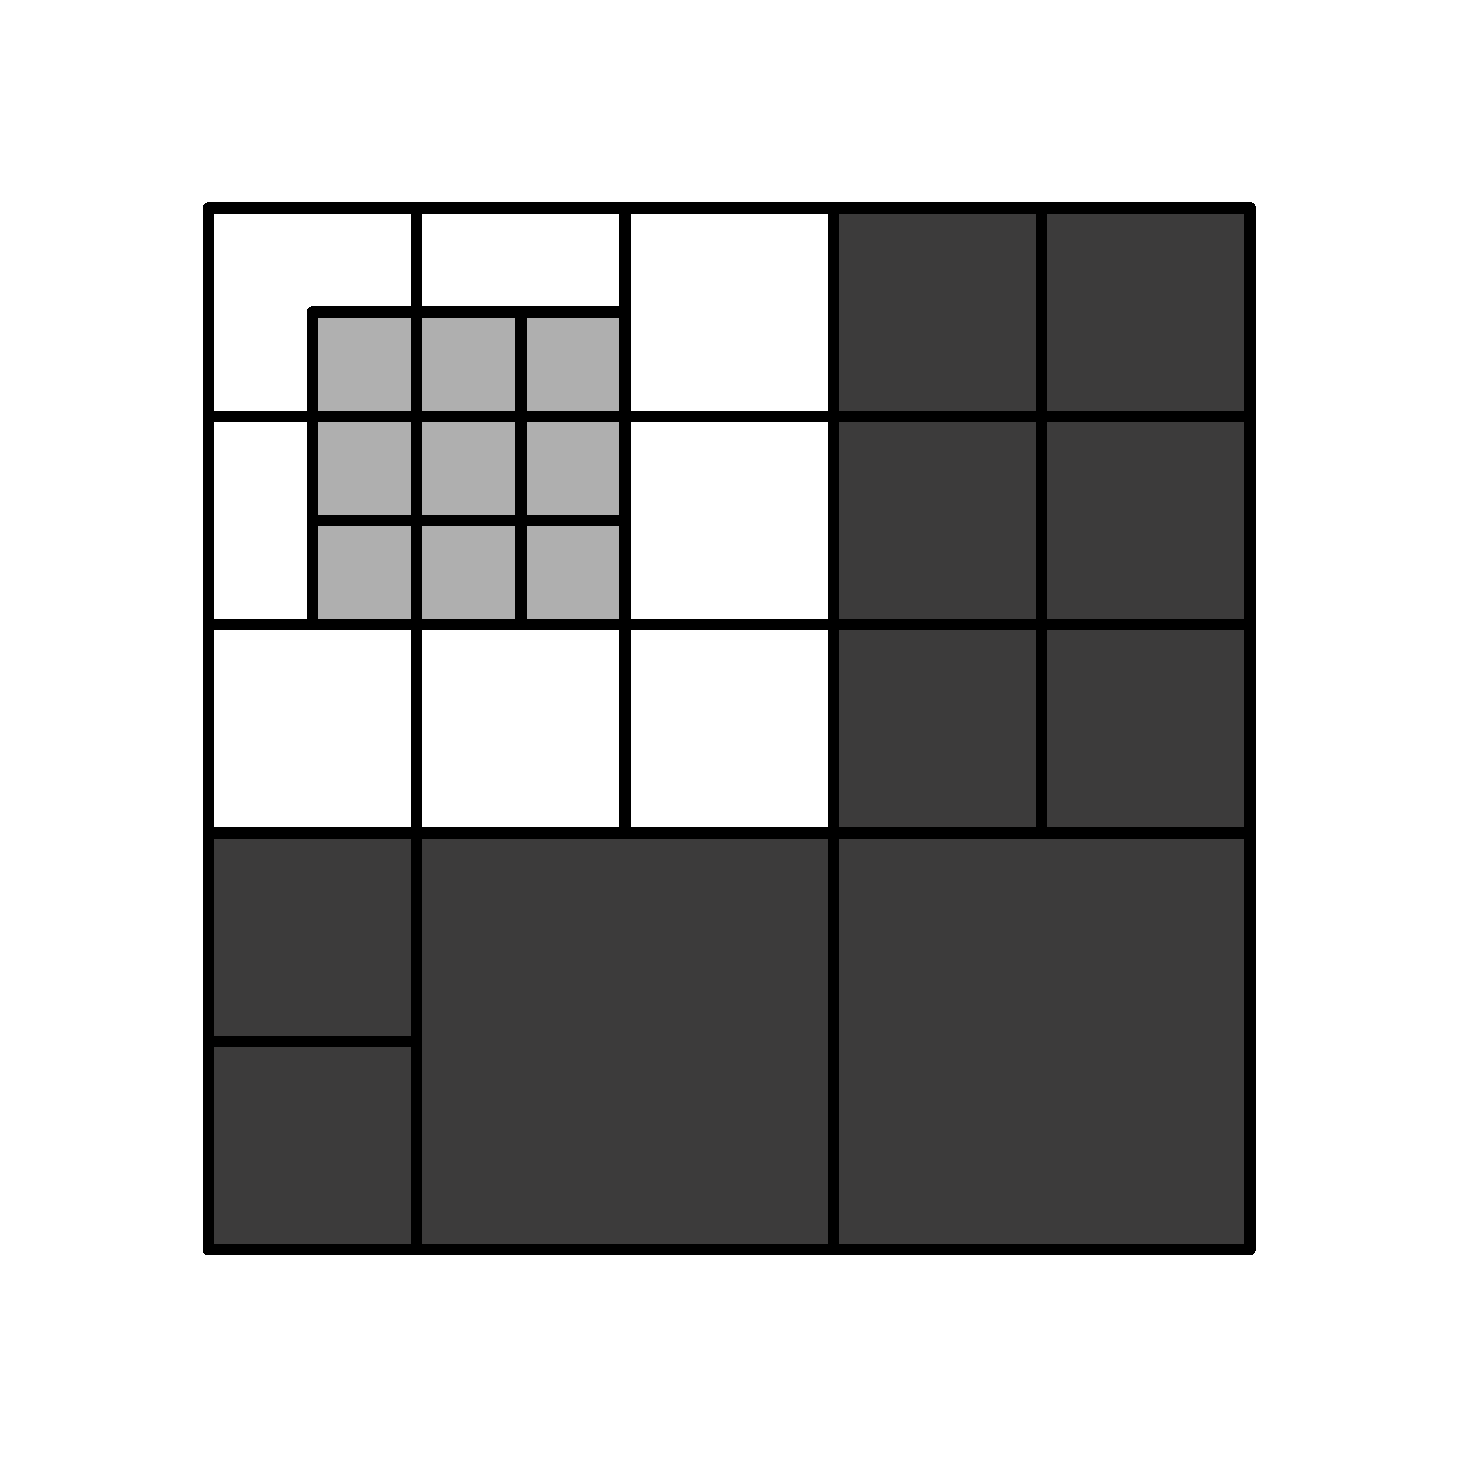
\includegraphics[width=.6\textwidth]{Images/N-body problems/FMMDecomp.pdf}};
    \begin{scope}[x={(image.south east)},y={(image.north west)}]
    \begin{scope}[x={(image.south east)},y={(image.north west)}]
        \node at (0.31,0.68) {$\underline{i}$};
    \end{scope}
    \end{scope}
\end{tikzpicture}
}
    \caption[Node $i$'s interactions for the original FMM algorithm.]{Node $i$'s interactions for the original FMM algorithm. The interaction with particles in the near neighbour nodes (light grey) will be computed on the subsequent division. The particles in the white boxes are in the interaction list of $i$ so will be computed through multipole expansions. Interaction of particles in the most distinct nodes (dark grey) has already been computed in previous divisions.}
    \label{fig:FMMDecomp}
\end{figure}

The tree is traversed downwards from level $2$ to the leaf nodes. Level $1$ and $2$ do not need to be considered as there are no node pairs that are well separated until at least three subdivisions are made. The multipole expansion (eq.~\ref{eq:FMMOuterSingle}) is used to compute the contribution to the potential of all particles in a node from other well-separated nodes. The interactions of particles in a node's current near neighbours need to be considered which cannot be done by a multipole expansion due to their proximity. However, considering the node on the level below containing the considered particle, by the above definitions, this node will have a new set of near and well-separated nodes. These well-separated nodes contain, by definition, particles which were in the near neighbour nodes and can now be considered by multipole expansions. This process is continued until the bottom of the tree is reached and where particle to particle interactions are considered as in the Barnes-Hut method. 

\begin{algorithm}
\caption{The exact $N \log N$ Algorithm}\label{alg:FMMNlogN}
\begin{algorithmic}
\State Decompose the domain into a tree structure until there is one particle per node
\For{For each particle $i$ traverse the tree in pre order (see \cref{appendix:Tree}) to compute total force on the particle}
    \State Decompose the domain into 16/64 nodes
    \State Compute the contribution of particles in nodes well separated from the node
    \State \; containing $i$ using multipole expansions.
    \Repeat
        \State Subdivide all nodes into 4/8 children nodes.
        \State For nodes in the interaction list of the node containing $i$ compute the 
        \State \; contribution of using multipole expansions
    \Until{One particle per node}
    \State Compute remaining interactions of near neighbour nodes directly
\EndFor
\end{algorithmic}
\end{algorithm}

This version of the Fast Multipole method computes in the same $\mathcal{O}(N\log N)$ as the Barnes-Hut method, however, it is capable of exact results due to the use of the multipole expansions. Numerically this is not possible as infinite terms are needed for each expansion, so the expansions are truncated to $p$ terms where each expansion has an error estimate of
\begin{equation*}
    \left|\phi(z)-Q \log (z)-\sum_{k=1}^{p} \frac{a_{k}}{z^{k}}\right| \leq A\left(\frac{1}{2}\right)^{p} \text{ where } A = \sum_{i=1}^{n} |q_i|
\end{equation*}
where $n$ is the number of particles involved in the expansion \cite{Beatson,Greengard1987ASimulations}. This means that at each level, $\mathcal{O}(N)$ amount of work needs to be done, each multipole expansion requires $\mathcal{O}(p)$ operations giving each level a complexity of $\mathcal{O}(Np)$. Assuming homogeneity, where the particles are evenly distributed, then there will be approximately $\mathcal{O}(\log N)$ levels giving the overall complexity as $\mathcal{O}(N\log N)$ with the total cost being $27Np\log N + 8N$ where the $8N$ is the number of direct interactions and the factor of $27$ comes from the maximum size of the interaction list. 

\subsubsection{\texorpdfstring{The $\mathcal{O}(N)$ Algorithm}{The O(N) Algorithm}} \label{subsec:OrderNFMM}
In order to reduce the algorithm from $\mathcal{O}(N\log N)$ to $\mathcal{O}(N)$ better use of the multipole expansions need to be made. Greengard and Rokhlin proposed to further expand the multipole expansions, this time locally around the centre of a node $z_0$ such that all particles in a node can be considered using a single expansion.
By translating equation \cref{eq:FMMOuterSingle} to the centre of the node and again summing over all charges, the expansion takes the form
\begin{equation}
\label{eq:FMMOuterMultiTrans1}
    \phi(z) = a_0\log(z-z_0) + \sum_{k=1}^\infty \frac{b_k}{(z-z_0)^k}
\end{equation}
A further Taylor expansion with respect to $z_0$ now obtains the multipole expansion of a set of potentials located in a circle of radius $R$ centred at $z_0$ for a point outside a circle of radius $R+|z_0|$ at the origin as
\begin{equation}
\label{eq:FMMOuterMultiTrans2}
\begin{gathered}
    \phi(z) = a_0\log(z) + \sum_{k=1}^\infty \frac{b_k}{z^k} \quad \text{ where } \\
    a_0 = \sum_{i=1}^n q_i \quad \text{ and } \quad b_k = -\frac{a_0 z_0^k}{k} + \sum_{l=1}^{k} a_l z_0^{k-l} \binom{k-1}{l-1}
\end{gathered}
\end{equation}
with $\binom{k}{l}$ being the binomial coefficients.

While \cref{eq:FMMOuterMulti,eq:FMMOuterMultiTrans1} allow for the calculation of the potential away from a cluster of particles, the potential inside a circle $D_1$ also needs to be calculated. Considering a group of charges inside a circle $D_2$ with radius $R$ centred at $z_0$, with $|z_0|>(c+1)R$ with $c>1$. The potential at the origin can be found using \cref{eq:FMMOuterMultiTrans1} and then the potential can be expanded locally about the origin to be able to calculate the potential at a point inside the circle $D_1$ of radius $R$ centred at the origin as
\begin{equation}
\label{eq:FMMInner}
\begin{gathered}
    \phi(z) = \sum_{k=0}^\infty \frac{b_k}{z^k} \quad \text{ where } \\
    b_0 = a_0\log(-z_0) + \sum_{l=1}^\infty \frac{a_l}{z_0^l}(-1)^l \text{ and } \\
    b_k = -\frac{a_0}{k\cdot z_0^k} + \sum_{l=1}^{k} \frac{a_l}{z_0^{l}} \binom{l+k-1}{l-1}(-1)^l, \text{ for } l>0.
\end{gathered}
\end{equation}
This is obtained through a Maclaurin expansion about the point $z$, the full derivation can be seen in Beatson and Greengard \cite{Beatson}. The centre of this expansion can be translated using the following relation
\begin{equation}
    \label{eq:LocalTranslation}
    \sum_{k=0}^p a_k(z-z_0)^p = \sum_{k=0}^{p} \left( \sum_{l=k}^p a_k \binom{l}{k})(-z_0)^{l-1} \right)z^k.
\end{equation}

\begin{figure}
    \centering
        \resizebox{.5\linewidth}{!}{\begin{tikzpicture}
    \node[anchor = south west,inner sep=0] (image) at (0,0) {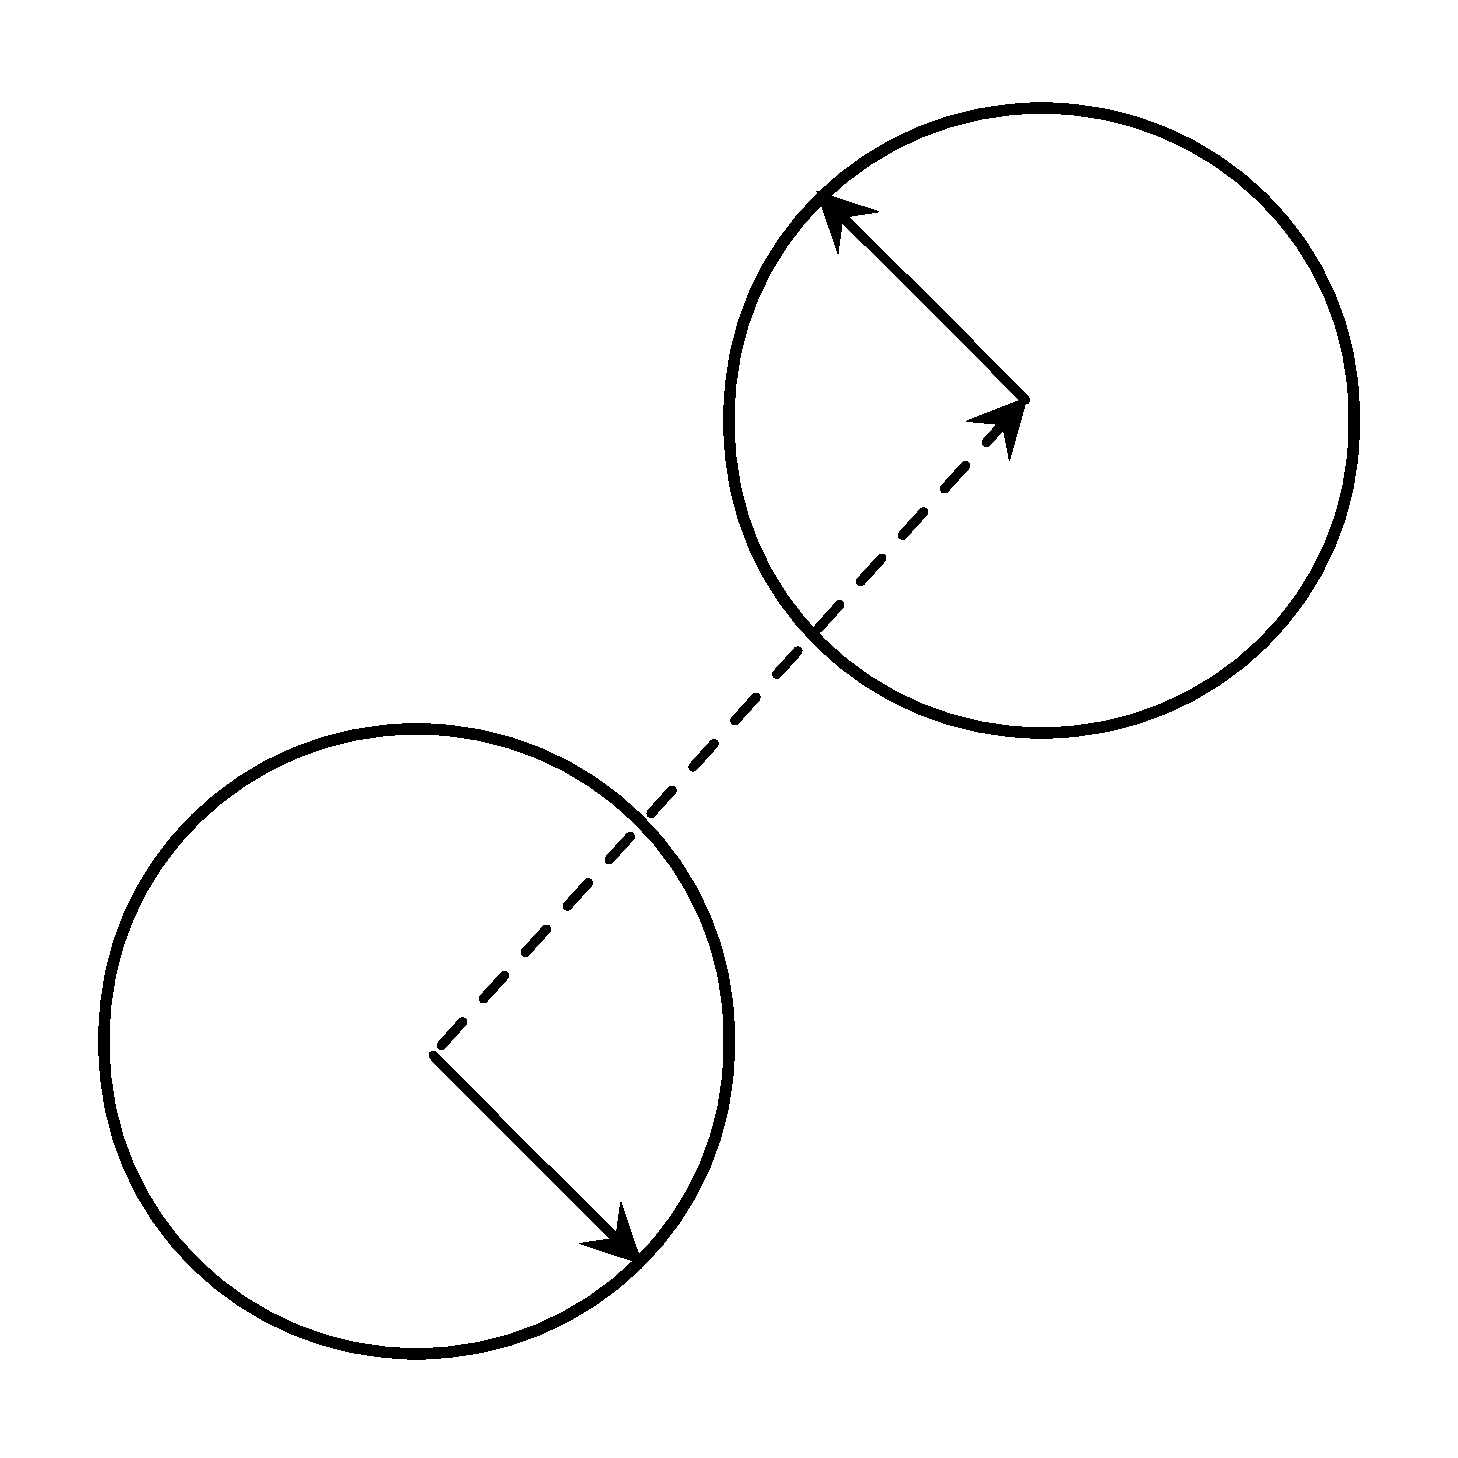
\includegraphics[width=.6\textwidth]{Images/KIFMM/Translation.pdf}};
    \begin{scope}[x={(image.south east)},y={(image.north west)}]
    \begin{scope}[x={(image.south east)},y={(image.north west)}]
        \node at (0.32,0.2) {$R$};
        \node at (0.70,0.8) {$R$};
        
        \node at (0.27,0.26) {$0$};
        \node at (0.74,0.73) {$z_0$};
        
        \node at (0.57,0.46) {$(c+1)R$};
        
        \node at (0.78,0.6) {$D_2$};
        \node at (0.2,0.4) {$D_1$};
    \end{scope}
    \end{scope}
\end{tikzpicture}
}
    \caption{Source charges $q_1,\dots,q_n$ are contained in the circle $D_2$. The corresponding expansion about $z_0$ converges inside $D_1$.}
    \label{fig:Translation}
\end{figure}

These expansions have the benefit of allowing for the evaluation of multipole expansions without the need to sum over all particles within that node. In particular, \cref{eq:FMMOuterMultiTrans2} allows for the calculation of the multipole expansion for all particles within a node by translating and summing over the expansions of the children nodes. In the downward pass, the method uses \cref{eq:LocalTranslation} to transmit the information of potentials outside of its near neighbours to its children.

The order $\mathcal{O}(N)$ is based on the $\mathcal{O}(N\log N)$ algorithm described in \cref{alg:FMMNlogN}, for simplicity we will only note the differences in the two methods here. Instead of decomposing the domain during the downward traversal of the tree, the tree is decomposed initially before any velocities are calculated. As the multipole expansions can be evaluated for any number of charges we only subdivide until there are at most $s$ particles per node at the finest level. As with the Barnes-Hut algorithm, the algorithm works from the bottom of the tree in post order. For leaf nodes, a truncated multipole expansion of $p$ terms is calculated based on the particles in the node. The expansions for all boxes in higher levels are then formed by shifting the expansions of all children nodes to the centre of the node and summing over coefficient terms.

Now that the upwards pass has formed a multipole expansion for each node based on all particles contained in it, the algorithm traverses down the tree computing node to node interactions. Instead of using the multipole expansions to calculate the effect of a node on a single particle, the method uses \cref{eq:FMMInner} to expand the multipole expansion of nodes in the interaction list into a local expansion which is valid inside the whole node. This expansion can then be shifted to the children of the node using \cref{eq:LocalTranslation} where the nodes in the childrens' interaction list is considered in the subsequent iteration.  After traversing the whole tree, each node on the highest level of a tree has a multipole expansion which takes into account all particles which are not in near neighbour nodes. The expansions can  be evaluated at all particle positions and then particle to particle interactions can be considered for all remaining particles. This three-step process is illustrated in \cref{fig:3Step} where the interactions between two well-separated nodes $A$ and $B$ are computed though the direct produce and through the use of multipole expansions.

\begin{figure}
    \centering
        \resizebox{.6\linewidth}{!}{\begin{tikzpicture}
    \node[anchor = south west,inner sep=0] (image) at (0,0) {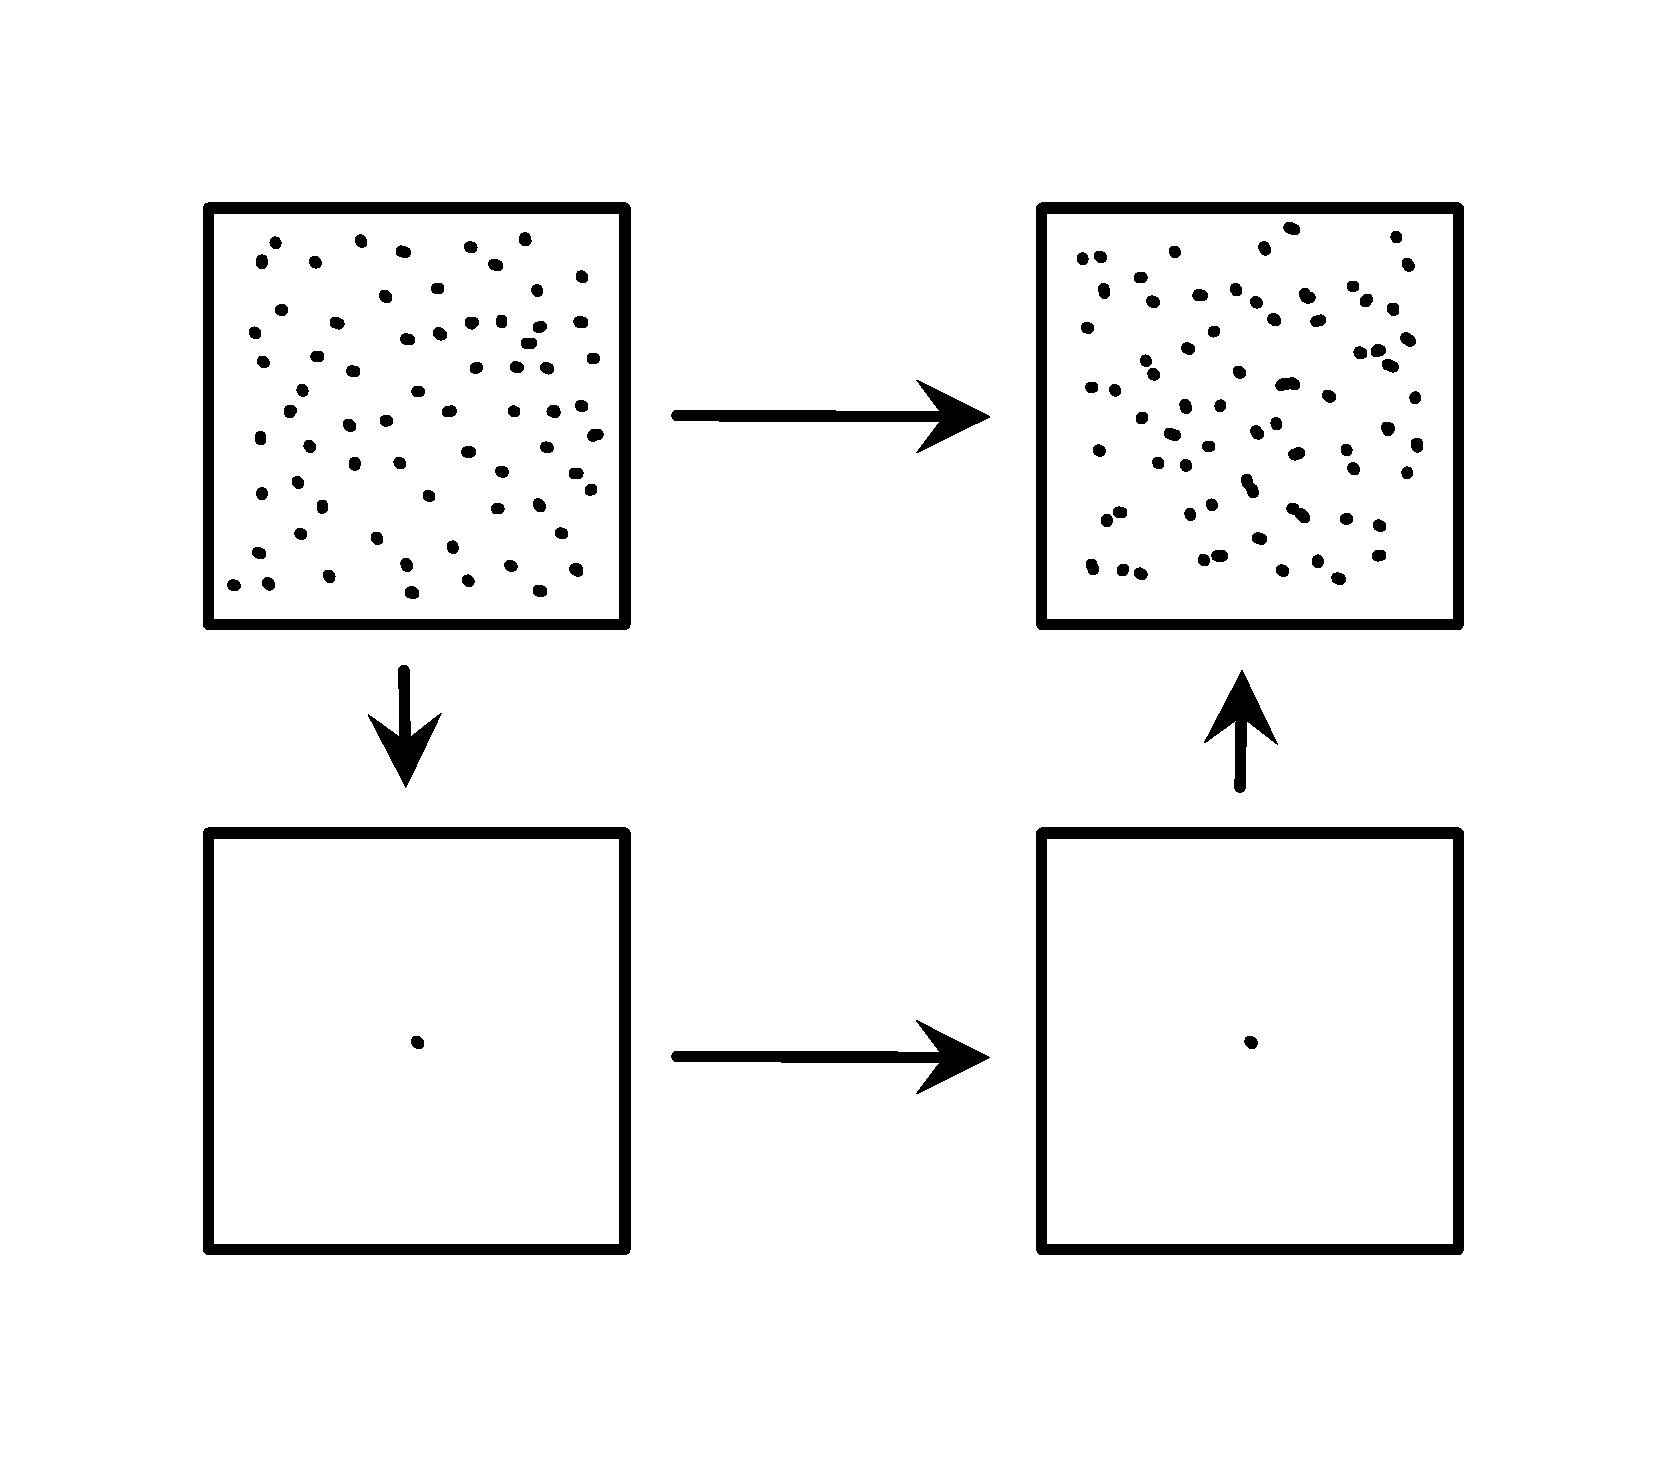
\includegraphics[width=.6\textwidth]{Images/KIFMM/3 Step.pdf}};
    \begin{scope}[x={(image.south east)},y={(image.north west)}]
    \begin{scope}[x={(image.south east)},y={(image.north west)}]
        \node at (0.25,0.9) {$A$};
        \node at (0.75,0.9) {$B$};
        
        \node at (0.25,0.22) {$C_A$};
        \node at (0.75,0.22) {$C_B$};
    
        \node at (0.5,0.78) {$\mathcal{O}(N^2)$};
        \node at (0.5,0.34) {$\mathcal{O}(1)$};
        \node at (0.35,0.5) {$\mathcal{O}(N)$};
        \node at (0.65,0.5) {$\mathcal{O}(N)$};
    \end{scope}
    \end{scope}
\end{tikzpicture}
}
    \caption[A diagram illustrating the three-step process FMM uses to reduce the complexity of $N$-body interactions from $\mathcal{O}(N^2)$ to $\mathcal{O}(N)$.]{A diagram illustrating the three-step process FMM uses to reduce the complexity of $N$-body interactions from $\mathcal{O}(N^2)$ to $\mathcal{O}(N)$. Assuming nodes $A$ and $B$ both have $N$ particles then directly computing the interaction takes $\mathcal{O}(N^2)$ operations. Taking the three-step process of computing the multipole expansion, translating the expansion and evaluation at the target points requires $\mathcal{O}(N)$ operations.
    }
    \label{fig:3Step}
\end{figure}

This three-step approach for calculating the interaction between two boxes yields an algorithm with total complexity $\mathcal{O}(N)$. In two dimensions the upwards pass takes $\mathcal{O}(Np)$ operations to calculate the multipole expansions for each node, $\mathcal{O}(29 \left(\frac{N}{s}\right) p^2)$ to shift the expansions between nodes, $\mathcal{O}(Np)$ operations to evaluate the local expansions and finally $\mathcal{O}(9Ns)$ operations to compute the near neighbour interactions. In three dimensions the total number of operations is of the order of $189\left(\frac{N}{s}\right)p^4 + 2Np^2 + 27Ns$. This means that the cost of increasing the accuracy of the original FMM algorithm in three dimensions grows to $\mathcal{O}(p^4)$, however, more recent work on the highly analytical structure of the FMM algorithm has allowed for the reduction of the cost of higher-order multipole expansions. Through the rotation of the nodes the work needed to translate the expansions has been decreased to $\mathcal{O}(p^4)$ to $\mathcal{O}(p^3)$ \cite{Greengard1997ADimensions,Hrycak1998AnFields} and even to $\mathcal{O}(p^2)$ by diagonalising the translations \cite{Berman2006Grid-MultipoleCalculations,Elliott1996FastAlgorithm}, however, these introduce numerical instabilities into the algorithm. The latest generation of FMMs are based on combining multipole expansions with plane wave expansions \cite{Greengard1997ADimensions,Hrycak1998AnFields} allowing for numerically stable calculations in three dimensions with a dependence on $p$ of only $\mathcal{O}(p^2)$ calculations. 

The multipole expansions presented here are derived from the two dimensional Coulomb potential and are taken from \cite{Beatson,Greengard1987ASimulations}. Adaptation to three dimensional systems proves more analytically complicated but follows the same structure as the two dimensional case. Derivation of the multipole expansions in three dimensions typically involves the use of spherical harmonics, and the translations are more computationally complicated to evaluate. The adaptions to the algorithm can be seen in detail along with the full derivation of the expansions, translations and error estimates, in Greengard and Rokhlin (1987) \cite{Greengard1987ASimulations} and Beatson and Greengard (1997) \cite{Beatson}. The FMM is widely used and has been deployed in stellar dynamics as an improvement to the Barnes-Hut algorithm \cite{Dehnen2014ADynamics}, in heat conduction \cite{Watschinger2021AEquation} and in non regularised Stokes flow \cite{Selmi2007FastComplexity,Tornberg2008}. The only problem with the standard FMM algorithms is the need to calculate multipole expansions for each kernel independently which can be difficult in cases such as the case of the stokeslet kernel. We will now look at an adaption to the FMM algorithm to create a Kernel Independent Fast Multipole (KIFMM) algorithm proposed by Ying \cite{Ying2004,Ying2005}.